%
% This work is licensed under a Creative Commons Attribution-ShareAlike 4.0 International License.
% http://creativecommons.org/licenses/by-sa/4.0/
%
\documentclass{beamer}
\usetheme[pageofpages=of,% String used between the current page and the
                         % total page count.
          bullet=circle,% Use circles instead of squares for bullets.
          titleline=true,% Show a line below the frame title.
          alternativetitlepage=true,% Use the fancy title page.
	  titlepagelogo=images/logoM-circl-Forensics.png,% Logo for the first page.
%          watermark=watermark-polito,% Watermark used in every page.
%          watermarkheight=100px,% Height of the watermark.
%          watermarkheightmult=4,% The watermark image is 4 times bigger
                                % than watermarkheight.
          ]{Torino}

\usepackage[utf8]{inputenc}
\usepackage{listings}
\usepackage{color}
\usepackage[font=small,labelfont=bf]{caption}
\usepackage{transparent}
\usepackage{siunitx}

\usepackage[norndcorners,customcolors]{hf-tikz}
\hfsetbordercolor{yellow}
\hfsetfillcolor{yellow}

\lstset{ 
  backgroundcolor=\color{white},   % choose the background color; you must add \usepackage{color} or \usepackage{xcolor}
  basicstyle=\footnotesize,        % the size of the fonts that are used for the code
  breakatwhitespace=false,
}


\author{CIRCL \emph{TLP:CLEAR}}
\title{CIRCL - Digital Forensics 1.0.1}
\subtitle{Introduction: Post-mortem Digital Forensics}
\institute{info@circl.lu}
\date{December, 2024}



\begin{document}
\begin{frame}[t,plain]
\titlepage
\end{frame}


\begin{frame}
  \frametitle{Overview}
  \begin{itemize}
  \item[]
      \begin{enumerate}
          \item Introduction
          \item Information
          \item Disk Acquisition
          \item Disk Cloning / Disk Imaging
          \item Disk Analysis
          \item Forensics Challenges
          \item Bibliography and Outlook
      \end{enumerate}
  \end{itemize}
\end{frame}


%
% This work is licensed under a Creative Commons Attribution-ShareAlike 4.0 International License.
% http://creativecommons.org/licenses/by-sa/4.0/
%

% DO NOT COMPILE THIS FILE DIRECTLY!
% This is included by the other .tex files.


\begin{frame}
    \includegraphics[scale=0.3]{images/logo-circl-Forensics.png}
    \begin{itemize}
        \item[]
        \item[]
        \item[] 1. Introduction
    \end{itemize}
\end{frame}


\begin{frame}
  \frametitle{1.1 Admin default behaviour}
  \begin{itemize}
    \item Get operational asap:
    \begin{itemize}
      \item Re-install
      \item Re-image
      \item Restore from backup
      \item[] $\to$ Destroy of evidences
      \item[]
    \end{itemize}
    \item Analyse the system on his own:
    \begin{itemize}
      \item Do some investigations
      \item Install and run (several) AV
      \item Apply updates for OS and Apps
      \item[] $\to$ Create big noise
      \item[] $\to$ Overwrite evidences
      \item[]
    \end{itemize}
    \item[] $\to$ Negative impact on forensics
  \end{itemize}
\end{frame}


\begin{frame}
  \frametitle{1.2 Preservation of evidences}
  \begin{itemize}
      \item Finding answers:
      \begin{itemize}
          \item[] $\to$ Is there an incident
          \item[] $\to$ System involved at all
          \item[] $\to$ If yes, how and when
          \item[] $\to$ System compromised
          \item[] $\to$ Malware/RAT involved
          \item[] $\to$ Persistence mechanisms
          \item[] $\to$ Root cause of the compromise
          \item[] $\to$ Lateral movement inside LAN
          \item[] $\to$ Access sensitive data
          \item[] $\to$ Data exfiltration
          \item[] $\to$ Illegal content
          \item[]
      \end{itemize}
      \item Legal case:
      \begin{itemize}
	  \item[] $\to$ Collect \& safe evidences
	  \item[] $\to$ Witness testimony for court
      \end{itemize}
  \end{itemize}
\end{frame}


\begin{frame}
  \frametitle{1.2 Preservation of evidences}
  \begin{itemize}
      \item A cyclic redundancy check (CRC) is not sufficient:
      \begin{itemize}
          \item Example: Checksum
          \begin{itemize}
		  \item[] 4711 $\to$ 13
          \end{itemize}
          \item Example: Collision
          \begin{itemize}
		  \item[] 12343 $\to$ 13
		  \item[] 
          \end{itemize}
      \end{itemize}
      \item Cryptographic hash function:
      \begin{itemize}
          \item Output always same fixed size
	  \item Deterministic: if $m = m \to h(m) = h(m)$
	  \item 1 Bit change in m $\to$ max. change in $h(m)$
	  \item One way function: For $h(m)$ impossible to find m
	  \item Simple collision resistance: For given $h(m1)$ hard to find $h(m2)$
	  \item Strong collision resistance: For any $h(m1)$ hard to find $h(m2)$
	  \item[]
      \end{itemize}
  \end{itemize}
\end{frame}


\begin{frame}
  \frametitle{1.3 Forensics Science}
  \begin{itemize}
    \item Classical forensic
    \begin{itemize}
      \item[] Locard's exchange principle
      \item[] {\scriptsize \url{https://en.wikipedia.org/wiki/Locard's\_exchange\_principle}}
    \end{itemize}
    \item[]
    \item Write down everything you see, hear, smell and do
    \item[]
    \item Chain of custody
    \begin{itemize}
        \item[] $\to$ {\scriptsize \url{https://csrc.nist.gov/glossary/term/chain\_of\_custody}}
        \item[] $\to$ {\scriptsize \url{https://www.nist.gov/document/sample-chain-custody-formdocx}}
    \end{itemize}
    \item[]
    \item Scope of the analysis
  \end{itemize}
\end{frame}


\begin{frame}
  \frametitle{1.3 Forensics Science}
  \begin{itemize}
      \item[] CPU registers $\to$ nanoseconds
      \item[] CPU cache $\to$ nanoseconds
      \item[] RAM memory $\to$ tens of nanoseconds
      \item[] Network state $\to$ milliseconds
      \item[] Processes running $\to$ seconds
      \item[] Disk, system settings, data $\to$ minutes
      \item[] External disks, backup $\to$ years
      \item[] Optical storage, printouts $\to$ tens of ears
      \item[] 
      \item[] $\to$ \url{https://www.circl.lu/pub/tr-22/}
  \end{itemize}
\end{frame}


\begin{frame}
  \frametitle{1.4 Forensic disciplines}
  \begin{itemize}
      \item Post-mortem Analysis
        \begin{itemize}
            \item[] $\to$ \url{https://www.circl.lu/pub/tr-22/}
            \item[] $\to$ \url{https://www.circl.lu/pub/tr-30/}
        \end{itemize}
      \item Memory Forensics
        \begin{itemize}
            \item[] $\to$ \url{https://www.circl.lu/pub/tr-22/}
            \item[] $\to$ \url{https://www.circl.lu/pub/tr-30/}
        \end{itemize}
      \item Reverse Engineering
      \item Code-Deobfuscation
      \item Network Forensics
      \item Mobile Forensics
      \item Cloud Forensics
  \end{itemize}
\end{frame}


\begin{frame}
  \frametitle{1.5 First Responder: Be prepared}
  \begin{itemize}
      \item Prepare your toolbox
      \begin{itemize}
          \item Write Blocker
          \item Photo camera
          \item Flash light, magnifying glasses
          \item Labelling device, labels, tags, stickers
          \item Toolkit, screwdriver kits
          \item Packing boxes, bags, faraday bag
          \item Cable kits, storage devices
          \item Anti-static band, network cables
          \item Pens, markers, notepads
          \item[] $\to$ Chain of custody
          \item Mouse jiggler
	  \item[]
      \end{itemize}
      \item Talk with people; Take notes
      \item Identify potential evidences (Computer, devices, paper, ...)
  \end{itemize}
\end{frame}


\begin{frame}
  \frametitle{1.5 First Responder: First steps}
  \begin{itemize}
      \item Powered-on versus powered-off
      \begin{itemize}
	  \item Shutdown: Lost of live (memory) data
          \item Pull power: Corrupt file system
          \item Live analysis: Modify memory and disk
          \item Live analysis: Working with compromised binaries?
	  \item[]
      \end{itemize}
      \item USB stick $\to$ \url{https://www.circl.lu/pub/tr-30/}
      \begin{itemize}
          \item 256 GB USB3
          \item File system: exFAT
          \item Memory dump: Comae-Toolkit
          \item Memory and Live Acquisition: FTK Imager Lite
          \item Encrypted Disk Detector - Edd
          \item Security Scanner: Nmap command line
          \item Sysinternals Suite
      \end{itemize}
  \end{itemize}
\end{frame}


\begin{frame}
  \frametitle{1.5 First Responder: Live response}
  \begin{enumerate}
	  \item Isolate system from (WiFi) network
      \item Perform memory dump
      \item In case of a live analysis:
      \begin{itemize}
          \item[] $\to$ System time
          \item[] $\to$ Logged-on users
          \item[] $\to$ Open files
          \item[] $\to$ Network -connections -status
          \item[] $\to$ Process information -memory
          \item[] $\to$ Process / port mapping
          \item[] $\to$ Clipboard content
          \item[] $\to$ Services
          \item[] $\to$ Command history
          \item[] $\to$ Mapped drives / shares
          \item[] $\to$ !!! Do not store information on the subject system !!!
      \end{itemize}
      \item Shutdown and do disk image (If possible)
      \item Logical image of live system $($Possible issues$)$
  \end{enumerate}
\end{frame}


\begin{frame}
  \frametitle{1.6 Post-mortem Analysis}
  \begin{itemize}
      \item Hardware layer \& acquisition
        \begin{itemize}
            \item[] Best copy (in the safe)
            \item[] Working copy (on a NAS)
            \item[] Working copy attached with Write Blocker
            \item[] Disk volumes and partitions
            \item[] Simple tools: dmesg, dd, mount
            \item[]
        \end{itemize}
      \item Sector layer
        \begin{itemize}
            \item[] Carving: foremost, scalpel, testdisk/photorec
            \item[] String search
            \item[]
        \end{itemize}
      \item File system layer
        \begin{itemize}
            \item[] FAT, NTFS
            \item[] File system timeline
            \item[] Restore deleted files
            \item[]
        \end{itemize}
  \end{itemize}
\end{frame}


\begin{frame}
  \frametitle{1.7 Post-mortem Analysis}
  \begin{itemize}
      \item OS layer
        \begin{itemize}
            \item[] Registry
            \item[] Event logs
            \item[] Volume shadow copies
            \item[] Prefetch files
            \item[]
        \end{itemize}
      \item Application layer
        \begin{itemize}
            \item[] AV logs
            \item[] Browser history: IE, firefox, chrome
            \item[] Email
            \item[] Office files \& PDFs
            \item[]
        \end{itemize}
      \item Searching for malware
        \begin{itemize}
            \item[] TEMP folders
            \item[] Startup folders
            \item[] Windows tasks
            \item[]
        \end{itemize}
  \end{itemize}
\end{frame}


\begin{frame}
  \frametitle{1.8 Forensic Distributions}
  \begin{itemize}
      \item Commercial
        \begin{itemize}
            \item[] \href{https://www.guidancesoftware.com/encase-forensic}{EnCase Forensic}
            \item[] \href{https://www.f-response.com/}{F-Response}
            \item[] \href{https://accessdata.com/products-services/forensic-toolkit-ftk}{Forensic Toolkit}
            \item[] \href{http://www.e-fense.com/products.php}{Helix Enterprise}
            \item[] \href{http://www.x-ways.net/forensics/index-d.html}{X-Ways Forensics}
            \item[] \href{https://www.magnetforensics.com/magnet-axiom/}{Magnet Axiom}
            \item[]
        \end{itemize}
      \item Open source tools
        \begin{itemize}
            \item[] \href{https://www.kali.org/}{Kali Linux}
            \item[] \href{https://www.sans.org/tools/sift-workstation/}{SANS SIFT}
            \item[]
        \end{itemize}
      \item Consider using your favorite Linux and add tools
      \item Sometimes a Windows based VM could be helpful
  \end{itemize}
\end{frame}




%
% This work is licensed under a Creative Commons Attribution-ShareAlike 4.0 International License.
% http://creativecommons.org/licenses/by-sa/4.0/
%

% DO NOT COMPILE THIS FILE DIRECTLY!
% This is included by the other .tex files.


\begin{frame}
    \includegraphics[scale=0.3]{images/logo-circl-Forensics.png}
    \begin{itemize}
        \item[]
        \item[]
        \item[] 2. Information
    \end{itemize}
\end{frame}


\begin{frame}[fragile]
  \frametitle{2.1 Data in a binary system}
    \begin{itemize}
        \item BIT $\to$ Binary digit
        \item Data stored in binary form
            \begin{itemize}
                \item[] \begin{verbatim}x Bits --> 01010000011010010110111001100111 --> y Bits\end{verbatim}
                \item[] Bit x + 2 = 1
                \item[] Bit x + 3 = 0
                \item[] $\to$ What information is stored within this data?
            \end{itemize}
    \item[]
    \item \emph{"..... information is data arranged in a meaningful way for some perceived purpose ....."} $\to$ Interpretative rules
    \item[]
        \item Grouping, addressing and interpreting
            \begin{itemize}
                \item[] \begin{verbatim}-->   01010000   01101001   01101110   01100111   --> \end{verbatim}
                \item[] \begin{verbatim}      --------   --------   --------   -------- \end{verbatim}
                \item[] \begin{verbatim}-->   Byte 117   Byte 118   Byte 119   Byte 120   --> \end{verbatim}
            \end{itemize}
    \item[]
    \end{itemize}
\end{frame}


\begin{frame}[fragile]
  \frametitle{2.1 Data in a binary system}
    \begin{itemize}
        \item Grouping examples:
        \begin{itemize}
	    \item Nibble:\begin{footnotesize} \texttt{0101 0000 0110 1001 0110 1110 0110 0111} \end{footnotesize} 
            \item Byte:\begin{footnotesize} \texttt{01010000 01101001 01101110 01100111} \end{footnotesize}
            \item Word:\begin{footnotesize} \texttt{0101000001101001 0110111001100111} \end{footnotesize}
            \item Double Word:\begin{footnotesize} \texttt{01010000011010010110111001100111} \end{footnotesize}
	    \item[]
        \end{itemize}
        \item Interpreting:
        \begin{itemize}
	    \item Integer: (Signed, Unsigned)
	    \item Endian: (Big, Little)
            \item Floating Point
            \item Binary Coded Decimal, Packed BCD
	    \item Encoding: (ASCII, ISO8859, Unicode 16L, 16B, 32L, 32B)
	    \item Binary: (ELF, MZ, PE, GIF, JPEG, ZIP, PDF, OLE, ...)
            \item ...
        \end{itemize}
    \end{itemize}
\end{frame}


\begin{frame}[fragile]
  \frametitle{2.2 Number Systems}
    \begin{itemize}
        \item Decimal:
  \begin{lstlisting}[basicstyle=\tiny]
  2145
  ||||_   5 * 10^0 =      5
  |||__   4 * 10^1 =     40
  ||___   1 * 10^2 =    100
  |____   2 * 10^3 =  2,000
		      -----
                      2,145
  \end{lstlisting}
        \item Binary:
  \begin{lstlisting}[basicstyle=\tiny]
  1111
  ||||_   1 *  2^0 =      1
  |||__   1 *  2^1 =      2
  ||___   1 *  2^2 =      4
  |____   1 *  2^3 =      8
                     ------
                         15 = 1111
  \end{lstlisting}
        \item Hexadecimal:
  \begin{lstlisting}[basicstyle=\tiny]
  2A9F
  ||||_  15 * 16^0 =     15
  |||__  09 * 16^1 =    144
  ||___  10 * 16^2 =  2,560
  |____  02 * 16^3 =  8,192
                     ------
                     10,911 = 0x2A9F
  \end{lstlisting}
    \end{itemize}
\end{frame}


\begin{frame}[fragile]
  \frametitle{2.3 Interpreting binary data: Integer}
  \begin{verbatim}
  0 1 0 1 0 0 0 0
  ---------------
  | | | | | | | |_  0 * 2^0 =   0
  | | | | | | |___  0 * 2^1 =   0
  | | | | | |_____  0 * 2^2 =   0
  | | | | |_______  0 * 2^3 =   0
  | | | |_________  1 * 2^4 =  16
  | | |___________  0 * 2^5 =   0
  | |_____________  1 * 2^6 =  64
  |_______________  0 * 2^7 =   0
                              ---
                               80
  \end{verbatim}
\end{frame}


\begin{frame}[fragile]
  \frametitle{2.3 Interpreting binary data: Signed Integer}
  \begin{verbatim}
  1 0 1 1 1 1 1 1
  ---------------           Two's complement:
  | | | | | | | |

  0 1 0 0 0 0 0 0           1. Invert all single bits
  0 1 0 0 0 0 0 1           2. Add the value 1

    |           |

   64           1           3. Convert to Decimal
   --------------
              -65
  \end{verbatim}
\end{frame}


\begin{frame}[fragile]
  \frametitle{2.4 Exercise: Signed Integer Bytes}
  \begin{verbatim}
  1 1 0 1 1 1 0 0
  ---------------           Two's complement:
  | | | | | | | |

                            1. Invert all single bits
                            2. Add the value 1
    
      |     |

      ?     ?               3. Convert to Decimal
  ---------------
              -??
  \end{verbatim}
\end{frame}


\begin{frame}[fragile]
  \frametitle{2.4 Exercise: Signed Integer Bytes}
  \begin{verbatim}
  1 1 0 1 1 1 0 0
  ---------------           Two's complement:
  | | | | | | | |

  0 0 1 0 0 0 1 1           1. Invert all single bits
  0 0 1 0 0 1 0 0           2. Add the value 1
    
      |     |

     32     4               3. Convert to Decimal
  ---------------
              -36
  \end{verbatim}
\end{frame}


\begin{frame}[fragile]
  \frametitle{2.4 Exercise: Challenge on 1 byte signed Integer}
    \begin{itemize}
        \item Find biggest possible positive number
  \begin{lstlisting}[basicstyle=\tiny]
             		-->  
  \end{lstlisting}
        \item Find smalest possible positive number
  \begin{lstlisting}[basicstyle=\tiny]
              		-->  
  \end{lstlisting}
        \item Find biggest possible negative number
  \begin{lstlisting}[basicstyle=\tiny]
     	
     ---------	
     
              		-->  
     ---------	
  \end{lstlisting}
        \item Find smalest possible negative number
  \begin{lstlisting}[basicstyle=\tiny]
     
     ---------
              
              		--> 
     ---------
  \end{lstlisting}
    \end{itemize}
\end{frame}


\begin{frame}[fragile]
  \frametitle{2.4 Exercise: Challenge on 1 byte signed Integer}
    \begin{itemize}
        \item Find biggest possible positive number
  \begin{lstlisting}[basicstyle=\tiny]
     0111 1111		-->  127
  \end{lstlisting}
        \item Find smalest possible positive number
  \begin{lstlisting}[basicstyle=\tiny]
     0000 0000		-->    0
  \end{lstlisting}
        \item Find biggest possible negative number
  \begin{lstlisting}[basicstyle=\tiny]
     
     ---------	
     
              		--> 
     ---------	
  \end{lstlisting}
        \item Find smalest possible negative number
  \begin{lstlisting}[basicstyle=\tiny]
     
     ---------
    
              		--> 
     ---------
  \end{lstlisting}
    \end{itemize}
\end{frame}


\begin{frame}[fragile]
  \frametitle{2.4 Exercise: Challenge on 1 byte signed Integer}
    \begin{itemize}
        \item Find biggest possible positive number
  \begin{lstlisting}[basicstyle=\tiny]
     0111 1111		-->  127
  \end{lstlisting}
        \item Find smalest possible positive number
  \begin{lstlisting}[basicstyle=\tiny]
     0000 0000		-->    0
  \end{lstlisting}
        \item Find biggest possible negative number
  \begin{lstlisting}[basicstyle=\tiny]
     1111 1111	
     ---------	
     0000 0000	
     0000 0001		-->   -1
     ---------	
  \end{lstlisting}
        \item Find smalest possible negative number
  \begin{lstlisting}[basicstyle=\tiny]
     1000 0000
     ---------
     0111 1111
     1000 0000		--> -128
     ---------
  \end{lstlisting}
    \end{itemize}
\end{frame}


\begin{frame}[fragile]
  \frametitle{2.5 From Bin to Hex}
    \begin{itemize}
        \item[]
        \item[] Example:
            \begin{itemize}
                \item[] \begin{verbatim} 0001 1000    0101 0101    0000 1111    1010 0110\end{verbatim}
                \item[] \begin{verbatim} ---------    ---------    ---------    ---------\end{verbatim}
		\item[] \begin{verbatim}    1 8          5 5          0 F          A 6   \end{verbatim}
                \item[] 
            \end{itemize}
        \item[]
        \item[] Exercise:
            \begin{itemize}
                \item[] \begin{verbatim} 1001 0110    1010 0101    0000 1111    1100 0011\end{verbatim}
                \item[] \begin{verbatim} ---------    ---------    ---------    ---------\end{verbatim}
                \item[] \begin{verbatim}                                                 \end{verbatim}
                \item[] 
            \end{itemize}
    \end{itemize}
\end{frame}


\begin{frame}[fragile]
  \frametitle{2.5 From Bin to Hex}
    \begin{itemize}
        \item[]
        \item[] Exercise:
            \begin{itemize}
                \item[] \begin{verbatim} 1001 0110    1010 0101    0000 1111    1100 0011\end{verbatim}
                \item[] \begin{verbatim} ---------    ---------    ---------    ---------\end{verbatim}
                \item[] \begin{verbatim}                                                 \end{verbatim}
                \item[] 
            \end{itemize}
        \item[]
        \item[] Results:
            \begin{itemize}
                \item[] \begin{verbatim} 1001 0110    1010 0101    0000 1111    1100 0011\end{verbatim}
                \item[] \begin{verbatim} ---------    ---------    ---------    ---------\end{verbatim}
                \item[] \begin{verbatim}    9 6          A 5          0 F          C 3   \end{verbatim}
                \item[] 
            \end{itemize}
    \end{itemize}
\end{frame}


\begin{frame}[fragile]
  \frametitle{2.6 Big Endian and Little Endian}
	\begin{lstlisting}[basicstyle=\tiny]
Multibyte words:
	Example: 256 in Big Endian representation:

    2^:   15 14 13 12 11 10  9  8     7  6  5  4  3  2  1  0
           -  -  -  -  -  -  -  -     -  -  -  -  -  -  -  - 
  Data:    0  0  0  0  0  0  0  1     0  0  0  0  0  0  0  0 
           -  -  -  -  -  -  -  -     -  -  -  -  -  -  -  - 
Address:   10.000                     10.001 




            
Multibyte words:
	Example: 256 in Little Endian representation:

     2^:   7  6  5  4  3  2  1  0    15 14 13 12 11 10  9  8 
           -  -  -  -  -  -  -  -     -  -  -  -  -  -  -  - 
   Data:   0  0  0  0  0  0  0  0     0  0  0  0  0  0  0  1 
           -  -  -  -  -  -  -  -     -  -  -  -  -  -  -  - 
Address:   10.000                     10.001 
	\end{lstlisting}
\end{frame}


\begin{frame}[fragile]
  \frametitle{2.6 Exercise: Little Endian}
    \begin{itemize}
        \item[] Read and interpret this little endian 2 byte 'word'
            \begin{itemize}
                \item[] \begin{verbatim}        ------------- \end{verbatim}
                \item[] \begin{verbatim} 0x96A5 | 9 6 | A 5 | \end{verbatim}
                \item[] \begin{verbatim}        ------------- \end{verbatim}
                \item[] \begin{verbatim}                      \end{verbatim}
                \item[] \begin{verbatim}                      \end{verbatim}
                \item[] \begin{verbatim}                      \end{verbatim}
                \item[] \begin{verbatim}                      \end{verbatim}
                \item[] \begin{verbatim}                      \end{verbatim}
                \item[] \begin{verbatim}        ------------- \end{verbatim}
                \item[] \begin{verbatim} 0x     |     |     | =  \end{verbatim}
                \item[] \begin{verbatim}        ------------- \end{verbatim}
            \end{itemize}
    \end{itemize}
\end{frame}


\begin{frame}[fragile]
  \frametitle{2.6 Exercise: Little Endian}
    \begin{itemize}
        \item[] Read and interpret this little endian 2 byte 'word'
            \begin{itemize}
                \item[] \begin{verbatim}        ------------- \end{verbatim}
                \item[] \begin{verbatim} 0x96A5 | 9 6 | A 5 | \end{verbatim}
                \item[] \begin{verbatim}        ------------- \end{verbatim}
                \item[] \begin{verbatim}            \   /   \end{verbatim}
                \item[] \begin{verbatim}             \ /      \end{verbatim}
                \item[] \begin{verbatim}              X       \end{verbatim}
                \item[] \begin{verbatim}             / \      \end{verbatim}
                \item[] \begin{verbatim}            /   \   \end{verbatim}
                \item[] \begin{verbatim}        ------------- \end{verbatim}
                \item[] \begin{verbatim} 0xA596 | A 5 | 9 6 | = 42,390 \end{verbatim}
                \item[] \begin{verbatim}        ------------- \end{verbatim}
            \end{itemize}
    \end{itemize}
\end{frame}


\begin{frame}[fragile]
  \frametitle{2.6 Exercise: Little Endian}
    \begin{itemize}
        \item[] Read and interpret this little endian 'double word'
            \begin{itemize}
                \item[] \begin{verbatim}            ------------------------- \end{verbatim}
                \item[] \begin{verbatim} 0x1B2A0100 | 1 B | 2 A | 0 1 | 0 0 | \end{verbatim}
                \item[] \begin{verbatim}            ------------------------- \end{verbatim}
                \item[] \begin{verbatim}                                      \end{verbatim}
                \item[] \begin{verbatim}                                      \end{verbatim}
                \item[] \begin{verbatim}                                      \end{verbatim}
                \item[] \begin{verbatim}                                      \end{verbatim}
                \item[] \begin{verbatim}                                      \end{verbatim}
                \item[] \begin{verbatim}            ------------------------- \end{verbatim}
                \item[] \begin{verbatim} 0x         |     |     |     |     | =  \end{verbatim}
                \item[] \begin{verbatim}            ------------------------- \end{verbatim}
            \end{itemize}
    \end{itemize}
\end{frame}


\begin{frame}[fragile]
  \frametitle{2.6 Exercise: Little Endian}
    \begin{itemize}
        \item[] Read and interpret this little endian 'double word'
            \begin{itemize}
                \item[] \begin{verbatim}            ------------------------- \end{verbatim}
                \item[] \begin{verbatim} 0x1B2A0100 | 1 B | 2 A | 0 1 | 0 0 | \end{verbatim}
                \item[] \begin{verbatim}            ------------------------- \end{verbatim}
                \item[] \begin{verbatim}               \___   \   /   ___/    \end{verbatim}
                \item[] \begin{verbatim}                   \___\ /___/        \end{verbatim}
                \item[] \begin{verbatim}                    ___ X ___         \end{verbatim}
                \item[] \begin{verbatim}                ___/   / \   \___     \end{verbatim}
                \item[] \begin{verbatim}               /      /   \      \    \end{verbatim}
                \item[] \begin{verbatim}            ------------------------- \end{verbatim}
                \item[] \begin{verbatim} 0x00012A1B | 0 0 | 0 1 | 2 A | 1 B | = 76,315 \end{verbatim}
                \item[] \begin{verbatim}            ------------------------- \end{verbatim}
            \end{itemize}
    \end{itemize}
\end{frame}


\begin{frame}[fragile]
  \frametitle{2.7 Example: Other interpretation of binary data}
  \begin{itemize}
    \item[] BCD / PBCD
  \begin{verbatim}
     2        9        1       /     6  na    0  9
  -------- -------- --------   /   -------- -------- 
  00000010 00001001 00000001   /   01101010 00001001
                             
  \end{verbatim}
    \item[] ASCII
  \begin{verbatim}
  01110000  01101001  01101110  01100111
  --------  --------  --------  --------
    0x70      0x65      0x6E      0x67
     112       105       110       103
      p         i         n         g
  \end{verbatim}
  \end{itemize}
\end{frame}


\begin{frame}[fragile]
  \frametitle{2.8 Data structures: Exercise}
\begin{lstlisting}[basicstyle=\tiny]


	- Can you read this data?
	- Can you extract information out of this data?
	- Can you generate knowledge out of this data?


010001000100011001000101010000010000100000001110000000001111111
101110100011001010111001101110100001011100111010001111000011101
000010001001001000011001010110110001101100011011110010000001010
111011011110111001001101100011001000010001000001101010001000100
011001000101010000010000011100000001000000010000000001100100011
001100110100101110010001011100011011000110100010100100100010101
011010010010100101010101101001010000100111100101100100010101110
111100001101100011001010110011101101111001111010000101011111111
111111111111111111111111












_  
\end{lstlisting}
\end{frame}


\begin{frame}[fragile]
  \frametitle{2.8 Data structures: Organizing data}
\begin{lstlisting}[basicstyle=\tiny]
  0                       8                       16                      
 ------------------------------------------------------------------------- 
 |44|46|45|41|08|0E|00|FF|74|65|73|74|2E|74|78|74|22|48|65|6C|6C|6F|20|57|
 -------------------------------------------------------------------------
                                                        


  24                      32                      40
 -------------------------------------------------------------------------
 |6F|72|6C|64|22|0D|44|46|45|41|07|11|00|00|64|66|69|72|2E|36|34|52|45|5A|
 -------------------------------------------------------------------------
                   


 48                      56                       64
 -------------------------------------------------------------------------
 |4A|55|69|42|79|64|57|78|6C|65|67|6F|3D|0A|FF|FF|FF|FF|  |  |  |  |  |  |
 -------------------------------------------------------------------------










_  
\end{lstlisting}
\end{frame}


\begin{frame}[fragile]
  \frametitle{2.8 Data structures: Definition of the structure}
\begin{lstlisting}[basicstyle=\tiny]
  0                       8                       16                      
 ------------------------------------------------------------------------- 
 |44|46|45|41|08|0E|00|FF|74|65|73|74|2E|74|78|74|22|48|65|6C|6C|6F|20|57|
 -------------------------------------------------------------------------
                                                        


  24                      32                      40
 -------------------------------------------------------------------------
 |6F|72|6C|64|22|0D|44|46|45|41|07|11|00|00|64|66|69|72|2E|36|34|52|45|5A|
 -------------------------------------------------------------------------
                   


 48                      56                       64
 -------------------------------------------------------------------------
 |4A|55|69|42|79|64|57|78|6C|65|67|6F|3D|0A|FF|FF|FF|FF|  |  |  |  |  |  |
 -------------------------------------------------------------------------



Offset Size Description
     0    4 Header signature (ASCII: DFEA - Digital Forensics EDU Archive)
     4    1 Lenght of file name (Integer)
     5    2 Lenght of data (Little Endian)
     7    1 Type of data (Signed Integer)    (-1 = ASCII; 0 = base64 encoded)
     8   -- Variable file name (ASCII)
     9++ -- Data (Binary)
_    EOF  4 EOF signature (Binary: FF FF FF FF)
\end{lstlisting}
\end{frame}


\begin{frame}[fragile]
	\frametitle{2.8 Data structures: Apply structure}
\begin{lstlisting}[basicstyle=\tiny]
  0                       8                       16                      
 ------------------------------------------------------------------------- 
 |44|46|45|41|08|0E|00|FF|74|65|73|74|2E|74|78|74|22|48|65|6C|6C|6F|20|57|
 -------------------------------------------------------------------------
 |           |  |     |  |                                             


  24                      32                      40
 -------------------------------------------------------------------------
 |6F|72|6C|64|22|0D|44|46|45|41|07|11|00|00|64|66|69|72|2E|36|34|52|45|5A|
 -------------------------------------------------------------------------
                   


 48                      56                       64
 -------------------------------------------------------------------------
 |4A|55|69|42|79|64|57|78|6C|65|67|6F|3D|0A|FF|FF|FF|FF|  |  |  |  |  |  |
 -------------------------------------------------------------------------



Offset Size Description
     0    4 Header signature (ASCII: DFEA - Digital Forensics EDU Archive)
     4    1 Lenght of file name (Integer)
     5    2 Lenght of data (Little Endian)
     7    1 Type of data (Signed Integer)    (-1 = ASCII; 0 = base64 encoded)
     8   -- Variable file name (ASCII)
     9++ -- Data (Binary)
_    EOF  4 EOF signature (Binary: FF FF FF FF)
\end{lstlisting}
\end{frame}


\begin{frame}[fragile]
  \frametitle{2.8 Data structures: Read information}
\begin{lstlisting}[basicstyle=\tiny]
  0                       8                       16                      
 ------------------------------------------------------------------------- 
 |44|46|45|41|08|0E|00|FF|74|65|73|74|2E|74|78|74|22|48|65|6C|6C|6F|20|57|
 -------------------------------------------------------------------------
 | D  F  E  A|  |     |  |                                             


  24                      32                      40
 -------------------------------------------------------------------------
 |6F|72|6C|64|22|0D|44|46|45|41|07|11|00|00|64|66|69|72|2E|36|34|52|45|5A|
 -------------------------------------------------------------------------
                   


 48                      56                       64
 -------------------------------------------------------------------------
 |4A|55|69|42|79|64|57|78|6C|65|67|6F|3D|0A|FF|FF|FF|FF|  |  |  |  |  |  |
 -------------------------------------------------------------------------



Offset Size Description
     0    4 Header signature (ASCII: DFEA - Digital Forensics EDU Archive)
     4    1 Lenght of file name (Integer)
     5    2 Lenght of data (Little Endian)
     7    1 Type of data (Signed Integer)    (-1 = ASCII; 0 = base64 encoded)
     8   -- Variable file name (ASCII)
     9++ -- Data (Binary)
_    EOF  4 EOF signature (Binary: FF FF FF FF)
\end{lstlisting}
\end{frame}


\begin{frame}[fragile]
  \frametitle{2.8 Data structures: Read information}
\begin{lstlisting}[basicstyle=\tiny]
  0                       8                       16                      
 ------------------------------------------------------------------------- 
 |44|46|45|41|08|0E|00|FF|74|65|73|74|2E|74|78|74|22|48|65|6C|6C|6F|20|57|
 -------------------------------------------------------------------------
 | D  F  E  A| 8|     |  |                       |                      


  24                      32                      40
 -------------------------------------------------------------------------
 |6F|72|6C|64|22|0D|44|46|45|41|07|11|00|00|64|66|69|72|2E|36|34|52|45|5A|
 -------------------------------------------------------------------------
                   


 48                      56                       64
 -------------------------------------------------------------------------
 |4A|55|69|42|79|64|57|78|6C|65|67|6F|3D|0A|FF|FF|FF|FF|  |  |  |  |  |  |
 -------------------------------------------------------------------------



Offset Size Description
     0    4 Header signature (ASCII: DFEA - Digital Forensics EDU Archive)
     4    1 Lenght of file name (Integer)
     5    2 Lenght of data (Little Endian)
     7    1 Type of data (Signed Integer)    (-1 = ASCII; 0 = base64 encoded)
     8   -- Variable file name (ASCII)
     9++ -- Data (Binary)
_    EOF  4 EOF signature (Binary: FF FF FF FF)
\end{lstlisting}
\end{frame}


\begin{frame}[fragile]
  \frametitle{2.8 Data structures: Read information}
\begin{lstlisting}[basicstyle=\tiny]
  0                       8                       16                      
 ------------------------------------------------------------------------- 
 |44|46|45|41|08|0E|00|FF|74|65|73|74|2E|74|78|74|22|48|65|6C|6C|6F|20|57|
 -------------------------------------------------------------------------
 | D  F  E  A| 8|  14 |  |                


  24                      32                      40
 -------------------------------------------------------------------------
 |6F|72|6C|64|22|0D|44|46|45|41|07|11|00|00|64|66|69|72|2E|36|34|52|45|5A|
 -------------------------------------------------------------------------
                   


 48                      56                       64
 -------------------------------------------------------------------------
 |4A|55|69|42|79|64|57|78|6C|65|67|6F|3D|0A|FF|FF|FF|FF|  |  |  |  |  |  |
 -------------------------------------------------------------------------



Offset Size Description
     0    4 Header signature (ASCII: DFEA - Digital Forensics EDU Archive)
     4    1 Lenght of file name (Integer)
     5    2 Lenght of data (Little Endian)
     7    1 Type of data (Signed Integer)    (-1 = ASCII; 0 = base64 encoded)
     8   -- Variable file name (ASCII)
     9++ -- Data (Binary)
_    EOF  4 EOF signature (Binary: FF FF FF FF)
\end{lstlisting}
\end{frame}


\begin{frame}[fragile]
  \frametitle{2.8 Data structures: Read information}
\begin{lstlisting}[basicstyle=\tiny]
  0                       8                       16                      
 ------------------------------------------------------------------------- 
 |44|46|45|41|08|0E|00|FF|74|65|73|74|2E|74|78|74|22|48|65|6C|6C|6F|20|57|
 -------------------------------------------------------------------------
 | D  F  E  A| 8|  14 |-1|              


  24                      32                      40
 -------------------------------------------------------------------------
 |6F|72|6C|64|22|0D|44|46|45|41|07|11|00|00|64|66|69|72|2E|36|34|52|45|5A|
 -------------------------------------------------------------------------
                   


 48                      56                       64
 -------------------------------------------------------------------------
 |4A|55|69|42|79|64|57|78|6C|65|67|6F|3D|0A|FF|FF|FF|FF|  |  |  |  |  |  |
 -------------------------------------------------------------------------



Offset Size Description
     0    4 Header signature (ASCII: DFEA - Digital Forensics EDU Archive)
     4    1 Lenght of file name (Integer)
     5    2 Lenght of data (Little Endian)
     7    1 Type of data (Signed Integer)    (-1 = ASCII; 0 = base64 encoded)
     8   -- Variable file name (ASCII)
     9++ -- Data (Binary)
_    EOF  4 EOF signature (Binary: FF FF FF FF)
\end{lstlisting}
\end{frame}


\begin{frame}[fragile]
  \frametitle{2.8 Data structures: Apply informtion}
\begin{lstlisting}[basicstyle=\tiny]
  0                       8                       16                      
 ------------------------------------------------------------------------- 
 |44|46|45|41|08|0E|00|FF|74|65|73|74|2E|74|78|74|22|48|65|6C|6C|6F|20|57|
 -------------------------------------------------------------------------
 | D  F  E  A| 8|  14 |-1|                       |                      


  24                      32                      40
 -------------------------------------------------------------------------
 |6F|72|6C|64|22|0D|44|46|45|41|07|11|00|00|64|66|69|72|2E|36|34|52|45|5A|
 -------------------------------------------------------------------------
                   |


 48                      56                       64
 -------------------------------------------------------------------------
 |4A|55|69|42|79|64|57|78|6C|65|67|6F|3D|0A|FF|FF|FF|FF|  |  |  |  |  |  |
 -------------------------------------------------------------------------



Offset Size Description
     0    4 Header signature (ASCII: DFEA - Digital Forensics EDU Archive)
     4    1 Lenght of file name (Integer)
     5    2 Lenght of data (Little Endian)
     7    1 Type of data (Signed Integer)    (-1 = ASCII; 0 = base64 encoded)
     8   -- Variable file name (ASCII)
     9++ -- Data (Binary)
_    EOF  4 EOF signature (Binary: FF FF FF FF)
\end{lstlisting}
\end{frame}


\begin{frame}[fragile]
  \frametitle{2.8 Data structures: Interprete bytes}
\begin{lstlisting}[basicstyle=\tiny]
  0                       8                       16                      
 ------------------------------------------------------------------------- 
 |44|46|45|41|08|0E|00|FF|74|65|73|74|2E|74|78|74|22|48|65|6C|6C|6F|20|57|
 -------------------------------------------------------------------------
 | D  F  E  A| 8|  14 |-1| t  e  s  t  .  t  x t |                      


  24                      32                      40
 -------------------------------------------------------------------------
 |6F|72|6C|64|22|0D|44|46|45|41|07|11|00|00|64|66|69|72|2E|36|34|52|45|5A|
 -------------------------------------------------------------------------
                   |


 48                      56                       64
 -------------------------------------------------------------------------
 |4A|55|69|42|79|64|57|78|6C|65|67|6F|3D|0A|FF|FF|FF|FF|  |  |  |  |  |  |
 -------------------------------------------------------------------------



Offset Size Description
     0    4 Header signature (ASCII: DFEA - Digital Forensics EDU Archive)
     4    1 Lenght of file name (Integer)
     5    2 Lenght of data (Little Endian)
     7    1 Type of data (Signed Integer)    (-1 = ASCII; 0 = base64 encoded)
     8   -- Variable file name (ASCII)
     9++ -- Data (Binary)
_    EOF  4 EOF signature (Binary: FF FF FF FF)
\end{lstlisting}
\end{frame}


\begin{frame}[fragile]
  \frametitle{2.8 Data structures: Interprete bytes}
\begin{lstlisting}[basicstyle=\tiny]
  0                       8                       16                      
 ------------------------------------------------------------------------- 
 |44|46|45|41|08|0E|00|FF|74|65|73|74|2E|74|78|74|22|48|65|6C|6C|6F|20|57|
 -------------------------------------------------------------------------
 | D  F  E  A| 8|  14 |-1| t  e  s  t  .  t  x t | "  H  e  l  l  o     W


  24                      32                      40
 -------------------------------------------------------------------------
 |6F|72|6C|64|22|0D|44|46|45|41|07|11|00|00|64|66|69|72|2E|36|34|52|45|5A|
 -------------------------------------------------------------------------
   o  r  l  d  " CR|


 48                      56                       64
 -------------------------------------------------------------------------
 |4A|55|69|42|79|64|57|78|6C|65|67|6F|3D|0A|FF|FF|FF|FF|  |  |  |  |  |  |
 -------------------------------------------------------------------------



Offset Size Description
     0    4 Header signature (ASCII: DFEA - Digital Forensics EDU Archive)
     4    1 Lenght of file name (Integer)
     5    2 Lenght of data (Little Endian)
     7    1 Type of data (Signed Integer)    (-1 = ASCII; 0 = base64 encoded)
     8   -- Variable file name (ASCII)
     9++ -- Data (Binary)
_    EOF  4 EOF signature (Binary: FF FF FF FF)
\end{lstlisting}
\end{frame}


\begin{frame}[fragile]
  \frametitle{2.8 Data structures: Exercise: Your turn}
\begin{lstlisting}[basicstyle=\tiny]
  0                       8                       16                      
 ------------------------------------------------------------------------- 
 |44|46|45|41|08|0E|00|FF|74|65|73|74|2E|74|78|74|22|48|65|6C|6C|6F|20|57|
 -------------------------------------------------------------------------
 | D  F  E  A| 8|  14 |-1| t  e  s  t  .  t  x t | "  H  e  l  l  o     W


  24                      32                      40
 -------------------------------------------------------------------------
 |6F|72|6C|64|22|0D|44|46|45|41|07|11|00|00|64|66|69|72|2E|36|34|52|45|5A|
 -------------------------------------------------------------------------
   o  r  l  d  " CR|


 48                      56                       64
 -------------------------------------------------------------------------
 |4A|55|69|42|79|64|57|78|6C|65|67|6F|3D|0A|FF|FF|FF|FF|  |  |  |  |  |  |
 -------------------------------------------------------------------------



Offset Size Description
     0    4 Header signature (ASCII: DFEA - Digital Forensics EDU Archive)
     4    1 Lenght of file name (Integer)
     5    2 Lenght of data (Little Endian)
     7    1 Type of data (Signed Integer)    (-1 = ASCII; 0 = base64 encoded)
     8   -- Variable file name (ASCII)
     9++ -- Data (Binary)
_    EOF  4 EOF signature (Binary: FF FF FF FF)
\end{lstlisting}
\end{frame}


\begin{frame}[fragile]
	\frametitle{2.8 Data structures: Exercise: Solution}
\begin{lstlisting}[basicstyle=\tiny]
  0                       8                       16                      
 ------------------------------------------------------------------------- 
 |44|46|45|41|08|0E|00|FF|74|65|73|74|2E|74|78|74|22|48|65|6C|6C|6F|20|57|
 -------------------------------------------------------------------------
 | D  F  E  A| 8|  14 |-1| t  e  s  t  .  t  x t | "  H  e  l  l  o     W


  24                      32                      40
 -------------------------------------------------------------------------
 |6F|72|6C|64|22|0D|44|46|45|41|07|11|00|00|64|66|69|72|2E|36|34|52|45|5A|
 -------------------------------------------------------------------------
   o  r  l  d  " CR| D  F  E  A| 7|  17 | 0| d  f  i  r  .  6  4| R  E  Z


 48                      56                       64
 -------------------------------------------------------------------------
 |4A|55|69|42|79|64|57|78|6C|65|67|6F|3D|0A|FF|FF|FF|FF|  |  |  |  |  |  |
 -------------------------------------------------------------------------
   J  U  i  B  y  d  W  x  l  e  g  0  = NL|FF FF FF FF|


Offset Size Description
     0    4 Header signature (ASCII: DFEA - Digital Forensics EDU Archive)
     4    1 Lenght of file name (Integer)
     5    2 Lenght of data (Little Endian)
     7    1 Type of data (Signed Integer)    (-1 = ASCII; 0 = base64 encoded)
     8   -- Variable file name (ASCII)
     9++ -- Data (Binary)
_    EOF  4 EOF signature (Binary: FF FF FF FF)
\end{lstlisting}
\end{frame}


\begin{frame}
  \frametitle{2.9 Data, files, context}
    \begin{itemize}
        \item Sequence of Bits + Addressing + Interpretation $\to$ Information
        \item Where did you find the suspicious data?
            \begin{itemize}
                \item Binary inside TEMP folder
                \item Autorun folder
                \item Registry
                \item Browser history
                \item Command line history
            \end{itemize}
        \item [] $\to$ Data $\to$ Information $\to$ Knowledge
	\item[] 
        \item Information $\to$ Stored in files
	\item Files $\to$ Contains data
	\item Files $\to$ Data organized in data structures
	\item Files $\to$ Meta data describe files
        \item Files $\to$ File systems organize files and meta data
    \end{itemize}
\end{frame}










%
% This work is licensed under a Creative Commons Attribution-ShareAlike 4.0 International License.
% http://creativecommons.org/licenses/by-sa/4.0/
%

% DO NOT COMPILE THIS FILE DIRECTLY!
% This is included by the other .tex files.


\begin{frame}
    \includegraphics[scale=0.3]{images/logo-circl-Forensics.png}
    \begin{itemize}
        \item[]
        \item[]
        \item[] 3. Disk Acquisition
    \end{itemize}
\end{frame}


\begin{frame}[fragile]
  \frametitle{3.1 Storage devices / media}
    \begin{itemize}
        \item IBM 305 RAMAC - IBM 350 Disk Storage
        \begin{itemize}
            \item 1956: Random Access Method of Accounting and Control
            \item 152 x 172 x 63 cm; 500 kg
            \item 50.000 blocks of 100 Characters $\to$ 5MB
        \end{itemize}
    \end{itemize}
    \begin{figure}
        \includegraphics[scale=0.4, angle=0, trim=0 0 0 0]{images/IBM_305.jpeg}
        \captionsetup{labelformat=empty,labelsep=none}
        \transparent{0.4}%
        \caption[]{\tiny Image (c) www.chip.de - Image used solely for illustration purposes}
    \end{figure}
\end{frame}


\begin{frame}[fragile]
  \frametitle{3.1 Storage devices / media}
	\url{ftp://ftp.seagate.com/techsuppt/misc/jet.txt}
  \begin{lstlisting}[basicstyle=\tiny]
 The incredible feat of a read/write head:  Today's new generation of disc
 drives achieve the engineering equivalent of a Boeing 747 flying at MACH 4
 just two meters above the ground, counting each blade of grass as it flies
 over.  The read/write head floats at 12 millionths of an inch above the
 surface of the disc which is turning at 3,600 revolutions per minute.
 Read/write heads position precisely over information tracks which are 800
 millionths of an inch apart and the data is electronically recorded at
 20,000 bits per inch.



                                          __.
                                         / /   - - --
                                       /  /e
                                    ./   /e         /--u O O OO
                              /oAAAAAAAAAAAAAAAAAAA/ 
                            {  @@@  ooooooooooooooo @@'
                              \AAAAAA\AAAA\AAAAAAAAAA/
                                      ue\   \
                                         e\  \
                                            \_\. = = ==

AAAAAAAAAAAAAAAAAAAAAAAAAAAAAAAAAAAAAAAAAAAAAAAAAAAAAAAAAAAAAAAAAAAAA
  \end{lstlisting}
\end{frame}


\begin{frame}[fragile]
  \frametitle{3.1 Storage devices / media}
    \begin{itemize}
        \item Magnetic storage
        \begin{itemize}
            \item Tapes
            \item Floppy disks
            \begin{itemize}
                \item 8" - 1971 - 80KB
                \item 5.25" - 1976 - 360 KB
                \item 3.5" - 1984 - 1.2 MB / - 1986 - 1.44 MB
            \end{itemize}
            \item Hard disks
            \begin{itemize}
                \item IDE / EIDE, Firewire, PATA, SCSI
                \item SATA, SAS Serial attached SCSI, USB, Thunderbolt
            \end{itemize}
        \end{itemize}
        \item Optical storage
        \begin{itemize}
            \item Compact disks - CD
            \item Digital versatile disk - DVD
            \item Blu-ray disk
        \end{itemize}
        \item Non-volatile memory
        \begin{itemize}
            \item USB flash drive
            \item Solid state drive
            \item Flash memory cards
        \end{itemize}
    \end{itemize}
\end{frame}


\begin{frame}[fragile]
  \frametitle{3.2 Physical- / Logical layers}
  \begin{lstlisting}[basicstyle=\tiny]
	       Mass storage device
 ---------    ---------    ---------    ---------    Considerations: Disk duplication
| 8 TByte |  | 8 TByte |  | 8 TByte |  | 8 TByte |
 ---------    ---------    ---------    ---------      Speed USB2: 480 Mbit/s
     |            |            |            |            Capacity: 8 * 1024^4 * 8
     V            V            V            V            Duration: ~39 hours per disk
     RAID
   --------------------------------------------
  |  System  Data                              |       Speed USB3.1: 10 Gbit/s
  |  ----------------------------------------  |         Capacity: 24 * 1024^4 * 8
  | |  P1  |    P2 (24 TByte)                | |         Duration: ~5.5 hours per volume
  |  ----------------------------------------  |
   --------------------------------------------        (Theoretically)


A solution:
	- Local NAS
	- 10 GBit network
	- USB 3.1 / 3.2
	- 60+ TB mass storage
	- Virtual appliance
  \end{lstlisting}
\end{frame}


\begin{frame}[fragile]
  \frametitle{3.3 ATA Disks }
    \begin{itemize}
        \item ATA-3: Hard disk password
	\item[]
        \item ATA-4: HPA - Host Protected Area
        \begin{itemize}
            \item Not accessible by OS / user
            \item Persistent data - Survive format and re-installation
            \item Vendor area - Created by manufactur
            \item Diagnostics and recovery tools
            \item \texttt{READ\_NATIVE\_MAX\_ADDRESS}
        \end{itemize}
	\item[]
        \item ATA-6: DCO - Device Configuration Overlay
	\item[]
        \begin{itemize}
            \item Supports manufacturs with a layer of abstraction
              \begin{itemize}
                \item Use standard parts
		\item[] $\to$ To build different products
		\item[] $\to$ Example: Disks reports uniq amount of sectors
              \end{itemize}
        \end{itemize}
	\item[]
        \item ATA-7: Serial ATA
    \end{itemize}
\end{frame}


\begin{frame}[fragile]
  \frametitle{3.4 Demo: Hidden Sectors}
    \begin{itemize}
        \item New disk
\begin{lstlisting}[basicstyle=\tiny]
dmesg
    sd 1:0:0:0: [sdb] 3904981168 512-byte logical blocks: (2.00 TB/1.82 TiB)

hdparm -N /dev/sdb
    max sectors   = 3907029168/3907029168, ACCESSIBLE MAX ADDRESS disabled
\end{lstlisting}
        \item Create hidden message
\begin{lstlisting}[basicstyle=\tiny]
echo -n 'MySecret 123456' | dd of=/dev/sdb seek=3500000000

dd if=/bin/dd of=/dev/sdb seek=3500000001
     148+1 records in
     148+1 records out
     76000 bytes (76 kB, 74 KiB) copied, 0,022659 s, 3,4 MB/s
\end{lstlisting}
        \item Create HPA
\begin{lstlisting}[basicstyle=\tiny]
hdparm --yes-i-know-what-i-am-doing -N p3000000000 /dev/sdb
    setting max visible sectors to 3000000000 (permanent)
    max sectors   = 3000000000/3907029168, ACCESSIBLE MAX ADDRESS enabled

Power cycle your device after every ACCESSIBLE MAX ADDRESS
\end{lstlisting}
    \end{itemize}
\end{frame}


\begin{frame}[fragile]
  \frametitle{3.4 Demo: Hidden Sectors}
    \begin{itemize}
        \item Create partition and format
\begin{lstlisting}[basicstyle=\tiny]
dmesg
    sd 1:0:0:0: [sdb] 3000000000 512-byte logical blocks: (1.54 TB/1.40 TiB)

fdisk /dev/sdb
    primary
    2048
    2999999999

mkfs.ntfs -L CIRCL.DFIR -f /dev/sdb1
    Creating NTFS volume structures.
    mkntfs completed successfully. Have a nice day.
\end{lstlisting}
        \item Investigate disk layout
\begin{lstlisting}[basicstyle=\tiny]
fdisk -l /dev/sdb
    Device     Boot Start        End    Sectors  Size Id Type
    /dev/sdb1        2048 2999999999 2999997952  1,4T  7 HPFS/NTFS/exFAT
\end{lstlisting}
        \item Investigate last accessible sector
\begin{lstlisting}[basicstyle=\tiny]
dd if=/dev/sdb skip=2999999999 status=none| xxd
    00000000: eb52 904e 5446 5320 2020 2000 0208 0000  .R.NTFS    .....
      .......
    000001f0: 0000 0000 0000 0000 0000 0000 0000 55aa  ..............U.
\end{lstlisting}
    \end{itemize}
\end{frame}


\begin{frame}[fragile]
  \frametitle{3.4 Demo: Hidden Sectors}
    \begin{itemize}
        \item Try to access hidden message
\begin{lstlisting}[basicstyle=\tiny]
dd if=/dev/sdb skip=3500000000 count=1 | xxd
    dd: /dev/sdb: cannot skip: Invalid argument
    0+0 records in
\end{lstlisting}
        \item Resize HPA
\begin{lstlisting}[basicstyle=\tiny]
hdparm -N /dev/sdb
    max sectors   = 3000000000/3907029168, ACCESSIBLE MAX ADDRESS enabled

hdparm --yes-i-know-what-i-am-doing -N p3900000000 /dev/sdb
    max sectors   = 3900000000/3907029168, ACCESSIBLE MAX ADDRESS enabled

Power cycle your device after every ACCESSIBLE MAX ADDRESS
\end{lstlisting}
        \item Investigate disk layout and last sector
\begin{lstlisting}[basicstyle=\tiny]
fdisk -l /dev/sdb
    Device     Boot Start        End    Sectors  Size Id Type
    /dev/sdb1        2048 2999999999 2999997952  1,4T  7 HPFS/NTFS/exFAT

dd if=/dev/sdb skip=2999999999 status=none | xxd | less
dd if=/dev/sdb skip=3899999999 status=none | xxd | less
\end{lstlisting}
    \end{itemize}
\end{frame}


\begin{frame}[fragile]
  \frametitle{3.4 Demo: Hidden Sectors}
    \begin{itemize}
        \item Recover hidden message
\begin{lstlisting}[basicstyle=\tiny]
dd if=/dev/sdb skip=3500000000 count=1 status=none
    00000000: 4d79 5365 6372 6574 2031 3233 3435 3600  MySecret 123456.
\end{lstlisting}
	\item Recover hidden \texttt{dd} command
\begin{lstlisting}[basicstyle=\tiny]
dd if=/dev/sdb skip=$(( 3500000001*512 )) count=76000 bs=1 of=dd.exe

md5sum dd.exe
    36a70f825b8b71a3d9ba3ac9c5800683

md5sum /bin/dd
    36a70f825b8b71a3d9ba3ac9c5800683
\end{lstlisting}
        \item Feeback: kaplan(at)cert.at
\begin{lstlisting}[basicstyle=\tiny]
    https://www.schneier.com/blog/archives/2014/02/swap_nsa_exploi.html
    https://en.wikipedia.org/wiki/Host_protected_area
\end{lstlisting}
        \item How it works
\begin{lstlisting}[basicstyle=\tiny]
    IDENTIFY DEVICE
    SET MAX ADDRESS
    READ NATIVE MAX ADDRESS
    --> HPA aware software (like the BIOS)
\end{lstlisting}
    \end{itemize}
\end{frame}


\begin{frame}[fragile]
  \frametitle{3.5 Other Hidden Sectors}
    \begin{itemize}
        \item Service area, negative sectors
        \begin{itemize}
            \item Firmware
            \item Bad sectors
            \item ATA passwords
            \item[] \texttt{hdparm --security-unlock "myPassWD" /dev/sdb}
            \item SMART data
	    \item[]
        \end{itemize}
        \item Self-Monitoring, Analysis and Reporting Technology - SMART
        \begin{itemize}
            \item[] \texttt{apt install smartmontools}
            \item[] \texttt{smartctl -x /dev/sdb | less}
\begin{lstlisting}[basicstyle=\tiny]
.....
SMART Attributes Data Structure revision number: 16
Vendor Specific SMART Attributes with Thresholds:
ID# ATTRIBUTE_NAME          FLAGS    VALUE WORST THRESH FAIL RAW_VALUE
  1 Raw_Read_Error_Rate     POSR-K   200   200   051    -    0
  3 Spin_Up_Time            POS--K   234   233   021    -    3258
  4 Start_Stop_Count        -O--CK   100   100   000    -    679
  5 Reallocated_Sector_Ct   PO--CK   200   200   140    -    0
  7 Seek_Error_Rate         -OSR-K   200   200   000    -    0
  9 Power_On_Hours          -O--CK   095   095   000    -    3802
  .....
\end{lstlisting}
        \end{itemize}
    \end{itemize}
\end{frame}


\begin{frame}[fragile]
  \frametitle{3.6 Collecting information from devices}
    \begin{itemize}
        \item[] \texttt{hdparm -I /dev/sdb}
\begin{lstlisting}[basicstyle=\tiny]
ATA device, with non-removable media
        Model Number:       WDC WD20NPVT-00Z2TT0                    
        Serial Number:      WD-WX11A9269540
        Firmware Revision:  01.01A01
        Transport:          Serial, SATA 1.0a, SATA Rev 2.6, SATA Rev 3.0
Standards:
        Supported: 8 7 6 5 
        Likely used: 8
	.....
Security: 
        Master password revision code = 65534    supported
        not     enabled
        not     locked
        not     frozen
        not     expired: security count
        374min for SECURITY ERASE UNIT.
\end{lstlisting}
        \item[] \texttt{hdparm -I /dev/sda}
\begin{lstlisting}[basicstyle=\tiny]
...
Commands/features:
        Enabled Supported:
        ...
           *    Data Set Management TRIM supported (limit 8 blocks)
           *    Deterministic read ZEROs after TRIM
\end{lstlisting}
    \end{itemize}
\end{frame}














\begin{frame}[fragile]
  \frametitle{3.7 How is the device connected}
    \begin{itemize}
        \item Most relevant data with: \texttt{dmesg}
\begin{lstlisting}[basicstyle=\tiny]
dmesg -T
    .....
    [Mi Aug  1 13:06:11 2018] usb-storage 1-1:1.0: USB Mass Storage device detected
    [Mi Aug  1 13:06:11 2018] scsi host1: usb-storage 1-1:1.0
    [Mi Aug  1 13:06:13 2018] scsi 1:0:0:0: Direct-Access USB Flash DISK
    [Mi Aug  1 13:06:13 2018] sd 1:0:0:0: Attached scsi generic sg1 type 0
    [Mi Aug  1 13:06:13 2018] sd 1:0:0:0: [sdb] 15826944 512-byte logical blocks
\end{lstlisting}
        \item Enumerate host hardware
\begin{lstlisting}[basicstyle=\tiny]
lshw | less
    .....

lshw -businfo -class storage
    Bus info          Device           Class          Description
    =============================================================
    pci@0000:04:00.0                   storage        Samsung Electronics Co Ltd
    usb@2:3           scsi0            storage        
    usb@1:1           scsi1            storage

lshw -businfo -class disk
    Bus info          Device           Class          Description
    =============================================================
    scsi@0:0.0.0      /dev/sda         disk           SD/MMC CRW
                      /dev/sda         disk
    scsi@1:0.0.0      /dev/sdb         disk           2TB 2000FYYZ-01UL1B2
\end{lstlisting}
    \end{itemize}
\end{frame}


\begin{frame}[fragile]
  \frametitle{3.7 How is the device connected}
    \begin{itemize}
        \item Enumerate PCI bus
\begin{lstlisting}[basicstyle=\tiny]
lspci -d ::0106                      # List SATA controller

lspci -d ::0108                      # List NVME controller
    04:00.0 Non-Volatile memory controller: Samsung Electronics Co Ltd Device a808

lspci -d ::0C03                      # List USB, FW, ... controller
    00:14.0 USB controller: Intel Corporation Sunrise Point-LP USB 3.0 xHCI Controller (rev 21)
    3b:00.0 USB controller: Intel Corporation JHL6540 Thunderbolt 3 USB Controller (C step) [Alpine Ridge 4C 2016] (rev 02)
    3e:00.0 USB controller: Fresco Logic FL1100 USB 3.0 Host Controller (rev 10)
    40:00.0 USB controller: Fresco Logic FL1100 USB 3.0 Host Controller (rev 10)
\end{lstlisting}
        \item Enumerate block devices
\begin{lstlisting}[basicstyle=\tiny]
lsscsi -v

lsblk /dev/sdb
    NAME   MAJ:MIN RM  SIZE RO TYPE MOUNTPOINT
    sdb      8:16   0  1,8T  0 disk
     sdb1   8:17   0  1,8T  0 part /media/mich/031F0F30642CBB8B

lsblk -pd -o TRAN,NAME,SERIAL,VENDOR,MODEL,REV,WWN,SIZE,HCTL,SUBSYSTEMS /dev/sdb
    TRAN NAME     SERIAL          VENDOR   MODEL
    usb  /dev/sdb WD-WMC1P0H10ZEX WT055 WD 2000FYYZ-01UL1B2
             REV WWN                 SIZE HCTL       SUBSYSTEMS
            01.0 0x50014ee05979e023  1,8T 1:0:0:0    block:scsi:usb:pci
\end{lstlisting}
    \end{itemize}
\end{frame}


\begin{frame}[fragile]
	\frametitle{3.8 USB enumeration}
    \begin{itemize}
        \item List attached USB device
        \begin{itemize}
            \item USB bus
            \item Device address
            \item Vendor ID
            \item Product ID
            \item Product details
            \item[] ...
        \end{itemize}
        \item[] \texttt{lsusb}
\begin{lstlisting}[basicstyle=\tiny]
Bus 004 Device 001: ID 1d6b:0003 Linux Foundation 3.0 root hub
Bus 003 Device 001: ID 1d6b:0002 Linux Foundation 2.0 root hub
Bus 002 Device 002: ID 0bda:0328 Realtek Semiconductor Corp. 
Bus 002 Device 003: ID 1b1c:1a0e Corsair 
Bus 002 Device 004: ID 0951:162b Kingston Technology 
Bus 002 Device 001: ID 1d6b:0003 Linux Foundation 3.0 root hub
Bus 001 Device 004: ID 06cb:009a Synaptics, Inc. 
Bus 001 Device 003: ID 04f2:b61e Chicony Electronics Co., Ltd 
Bus 001 Device 001: ID 1d6b:0002 Linux Foundation 2.0 root hub
\end{lstlisting}
    \end{itemize}
\end{frame}


\begin{frame}[fragile]
	\frametitle{3.8 USB enumeration}
    \begin{itemize}
        \item[] \texttt{lsusb -t}
\begin{lstlisting}[basicstyle=\tiny]
/:  Bus 04.Port 1: Dev 1, Class=root_hub, Driver=xhci_hcd/2p, 10000M
/:  Bus 03.Port 1: Dev 1, Class=root_hub, Driver=xhci_hcd/2p, 480M
/:  Bus 02.Port 1: Dev 1, Class=root_hub, Driver=xhci_hcd/6p, 5000M
    |__ Port 1: Dev 4, If 0, Class=Mass Storage, Driver=usb-storage, 5000M
    |__ Port 2: Dev 3, If 0, Class=Mass Storage, Driver=uas, 5000M
    |__ Port 3: Dev 2, If 0, Class=Mass Storage, Driver=usb-storage, 5000M
/:  Bus 01.Port 1: Dev 1, Class=root_hub, Driver=xhci_hcd/12p, 480M
    |__ Port 8: Dev 3, If 1, Class=Video, Driver=uvcvideo, 480M
    |__ Port 8: Dev 3, If 0, Class=Video, Driver=uvcvideo, 480M
    |__ Port 9: Dev 4, If 0, Class=Vendor Specific Class, Driver=, 12M
\end{lstlisting}
        \item[] \texttt{lsusb  -v -d 0951:162b`}
\begin{lstlisting}[basicstyle=\tiny]
...
    Interface Descriptor:
      bLength                 9
      bDescriptorType         4
      bInterfaceNumber        0
      bAlternateSetting       0
      bNumEndpoints           2
      bInterfaceClass         8 Mass Storage
      bInterfaceSubClass      6 SCSI
      bInterfaceProtocol     80 Bulk-Only
...
\end{lstlisting}
    \end{itemize}
\end{frame}


\begin{frame}[fragile]
    \frametitle{3. usbmon \& wireshark}
	\frametitle{3.9 USB Interface monitoring}
    \begin{figure}
        \includegraphics[scale=0.18, angle=0, trim=0 0 0 0]{images/usbmon.png}\llap{\includegraphics[scale=0.27, trim = 0px 0px 0px 0px, angle=-5]{images/usbmon2.png}}
        % \includegraphics[scale=0.18, angle=0, trim=0 0 0 0]{images/usbmon.png}\llap{\includegraphics[height=5cm]{images/usbmon2.png}}
        \captionsetup{labelformat=empty,labelsep=none}
    \end{figure}
\end{frame}




%
% This work is licensed under a Creative Commons Attribution-ShareAlike 4.0 International License.
% http://creativecommons.org/licenses/by-sa/4.0/
%

% DO NOT COMPILE THIS FILE DIRECTLY!
% This is included by the other .tex files.


\begin{frame}
    \includegraphics[scale=0.3]{images/logo-circl-Forensics.png}
    \begin{itemize}
        \item[]
        \item[]
        \item[] 4. Disk Cloning / Disk Imaging
    \end{itemize}
\end{frame}


\begin{frame}[fragile]
  \frametitle{4.1 Disk cloning - imaging}
    \begin{itemize}
        \item Clone disk-2-disk
        \begin{itemize}
            \item Different sizes
            \item Wipe target disk!
        \end{itemize}
        \item Clone disk-2-image
        \begin{itemize}
            \item Clear boundaries
            \item One big file
            \item Break file into chunks
        \end{itemize}
        \item Image file format
        \begin{itemize}
            \item RAW
            \item AFF (Advanced Forensic Format)
            \item EWF (Expert Witness Format)
            \item Please no 3rd party formats
        \end{itemize}
        \item Write-Blockers
        \begin{itemize}
            \item Hardware
        \end{itemize}
    \end{itemize}
\end{frame}


\begin{frame}[fragile]
  \frametitle{4.2 Connecting devices}
    \begin{itemize}
        \item \texttt{udev} 
\begin{lstlisting}[basicstyle=\tiny]
udevadm info /dev/sda                 # userspace /dev
udevadm monitor
\end{lstlisting}
        \item \texttt{/dev/}
\begin{lstlisting}[basicstyle=\tiny]
/dev/sd*               # SCSI, SATA
/dev/hd*               # IDE. EIDE
/dev/md*               # RAID
/dev/nvme*n*           # NVME devices

/dev/sda1              # Partition 1 on disk 1
/dev/sda2              # Partition 2 on disk 1
...
\end{lstlisting}
        \item Block devices: Different level of access
        \begin{itemize}
            \item Attaching
            \item Mounting
        \end{itemize}
    \end{itemize}
\end{frame}


\begin{frame}[fragile]
  \frametitle{4.2 Read partition table}
    \begin{itemize}
        \item \texttt{dmesg} 
\begin{lstlisting}[basicstyle=\tiny]
[106834.127269] sd 6:0:0:0: Attached scsi generic sg1 type 0
[106834.127503] sd 6:0:0:0: [sdb] 15826944 512-byte logical blocks: (8.10 GB/7.54 GiB)
[106834.130380] sd 6:0:0:0: [sdb] Write Protect is off
\end{lstlisting}
        \item \texttt{fdisk -l circl-dfir.dd}
\begin{lstlisting}[basicstyle=\tiny]
Disk circl-dfir.dd: 1536 MB, 1536000000 bytes
4 heads, 7 sectors/track, 107142 cylinders, total 3000000 sectors
Units = sectors of 1 * 512 = 512 bytes
Sector size (logical/physical): 512 bytes / 512 bytes
I/O size (minimum/optimal): 512 bytes / 512 bytes
Disk identifier: 0x8f7e6594

        Device Boot      Start         End      Blocks   Id  System
circl-dfir.dd1            2048     3000000     1498976+   7  HPFS/NTFS/exFAT
\end{lstlisting}
        \item Exercise: Analyze output. Why \texttt{1498976}? $\to$ Conclusions?
    \end{itemize}
\begin{lstlisting}[basicstyle=\tiny]
End:     echo $(( 3000000 * 512 / 1024 ))           --> 1500000 KB
         echo $(( (3000000-2048) * 512 / 1024 ))    --> 1498976 KB

1498976: echo $(( 1498976 * 2 ))                    --> 2997952
\end{lstlisting}
\end{frame}


\begin{frame}[fragile]
  \frametitle{4.2 Mounting}
    \begin{itemize}
        \item \texttt{mount} 
\begin{lstlisting}[basicstyle=\tiny]
mkdir /mnt/ntfs                             # Create mount point
mount /dev/sdb1 /mnt/ntfs                   # Mounting

mount -o ro,remount /dev/sdb1 /mnt/ntfs     # Re-mounting

umount /mnt/ntfs                            # Un-mounting
umount /dev/sdb1                            # Also un-mounting


# Mounting readonly, no journaling, no executable
mount -o ro,noload,noexec /dev/sdb1 /mnt/ntfs
mount -o ro,noload,noexec,remount /dev/sdb1 /mnt/ntfs


# Mounting with offset. mounting from image files
mount -o ro,noload,noexec,offset=$((512*2048)) circl-dfir.dd /mnt/ntfs


# Mounting NTFS file systems
mount -o ro,noload,noexec,offset=$((512*2048)),
      show_sys_files,streams_interface=windows circl-dfir.dd /mnt/ntfs

\end{lstlisting}
    \end{itemize}
\end{frame}


\begin{frame}[fragile]
  \frametitle{4.3 dd - disk imaging rudimentary}
    \begin{itemize}
        \item[] Copy files from: \texttt{/mnt/ntfs/dd/}
\begin{lstlisting}[basicstyle=\tiny]
$ dd if=img_1.txt of=out_1.txt bs=512

     <input file>      <output file> <block size>
                                      (default)
3+0 records in
3+0 records out
1536 bytes (1.5 kB) copied, 0.000126 s, 12.2 MB/s

$ ll
-rw-rw-r-- 1 hamm hamm 1536 May 16 11:20 img_1.txt
-rw-rw-r-- 1 hamm hamm 1536 May 16 11:16 out_1.txt



$ dd if=img_2.txt of=out_2.txt bs=512
3+1 records in
3+1 records out
1591 bytes (1.6 kB) copied, 0.00016048 s, 9.9 MB/s

$ ll
-rw-rw-r-- 1 hamm hamm 1591 May 16 11:20 img_2.txt
-rw-rw-r-- 1 hamm hamm 1591 May 16 11:26 out_2.txt
\end{lstlisting}
    \end{itemize}
\end{frame}


\begin{frame}[fragile]
  \frametitle{4.3 dd - disk imaging rudimentary}
    \begin{itemize}
        \item[] Demo: \texttt{skip} and \texttt{count} options
\begin{lstlisting}[basicstyle=\tiny]
dd if=img_3.txt bs=512 skip=0 count=1 status=none | less
dd if=img_3.txt bs=512 skip=1 count=1 status=none | less
dd if=img_3.txt bs=512 skip=2 count=1 status=none | less
\end{lstlisting}
        \item[] Exercise: Play with \texttt{bs, skip} and \texttt{count} options
\begin{lstlisting}[basicstyle=\tiny]
dd if=img_3.txt bs=1 skip=$((512*3)) count=16 status=none
dd if=img_3.txt bs=16 skip=$((32*3)) count=1 status=none
\end{lstlisting}
        \item[] Exercise: \texttt{dd | xxd | less}
\begin{lstlisting}[basicstyle=\tiny]
dd if=img_3.txt bs=512 skip=3 count=1 status=none | xxd | less

    0000000: 4f76 6572 6865 6164 2031 3233 3435 3637  Overhead 1234567
    0000010: 3839 3020 204d 6573 7361 6765 2d31 2020  890  Message-1  
    0000020: 3039 3837 3635 3433 3231 2020 2020 2020  0987654321      
    0000030: 2020 2020 2020 20
\end{lstlisting}
        \item[] Exercise: Find the secret password behind sector 3
        \item[] 
    \end{itemize}
\end{frame}


\begin{frame}[fragile]
  \frametitle{4.3 dd - disk imaging rudimentary}
    \begin{itemize}
        \item[] Exercise: Continue an interrupted imaging process
\begin{lstlisting}[basicstyle=\tiny]
dd if=img_2.txt of=broken.raw bs=512 skip=0 count=2 status=none

ll  img_2.txt  ..... 1591 Aug 13 14:40 img_2.txt*
ll broken.raw  ..... 1024 Aug 13 15:05 broken.raw

dd if=img_2.txt of=broken.raw bs=512 skip=2 seek=2 status=none

md5sum  img_2.txt f319b1cc9d424a923a8c83c3e67185f1
md5sum broken.raw f319b1cc9d424a923a8c83c3e67185f1
\end{lstlisting}
        \item[] Error handling: Bad blocks
\begin{lstlisting}[basicstyle=\tiny]
$ dd if=img_3.txt of=out_3.txt bs=512 conv=noerror,sync
\end{lstlisting}
        \item[] Demo: Progress
\begin{lstlisting}[basicstyle=\tiny]
 Signaling: & and 'kill -10'
 Signaling: & and 'kill -USR1'
 Signaling: & and 'kill -USR1 $(pidof dd)'
 Option:    status=progress
\end{lstlisting}
    \end{itemize}
\end{frame}


\begin{frame}[fragile]
  \frametitle{4.4 Disk acquisition}
    \begin{itemize}
        \item Forensic features
        \begin{itemize}
            \item Progress monitoring
            \item Error handling \& logging
            \item Meta data
            \item Splitting output files \& support of forensic formats
            \item Cryptographic hashing \& verification checking
            \begin{itemize}
                \item[] \texttt{md5sum circl-dfir.dd} $\to$ \texttt{bd80672b9d1bef2f35b6e902f389e83}
                \item[] \texttt{sha1sum circl-dfir.dd} $\to$ \texttt{e5ffc7233a..........7e53b9f783}
            \end{itemize}
        \end{itemize}
        \item Tools
        \begin{itemize}
            \item dd
            \item ddrescue, gddrescue, dd\_rescue
            \item dc3dd - Department of Defense Cyber Crime Center
            \item dcfldd - Defense Computer Forensic Labs
	    \item rdd-copy, netcat, socat, ssh
            \item Guymager
        \end{itemize}
    \end{itemize}
\end{frame}


\begin{frame}[fragile]
  \frametitle{4.5 Exercise: dc3dd}
  \begin{lstlisting}[basicstyle=\tiny]
dc3dd if=/mnt/ntfs/carving/deleted.dd                   # Input file
      log=usb.log  -/                                   # Logging
      hash=md5 hash=sha1  -/                            # Hashing
      ofsz=$((8*1024*1024)) ofs=usb.raw.000             # Chunk files of 8MB


ls -l


cat usb.log


cat usb.raw.00* | md5sum                                # Verify hashes
cat usb.raw.00* | sha1sum


dc3dd wipe=/dev/sdx                                     # Wipe a drive
  \end{lstlisting}
\end{frame}


\begin{frame}[fragile]
  \frametitle{4.6 SuashFS as forensic container}
    \begin{itemize}
        \item Embedded systems
        \item Read only file system
        \item Supports very large files
        \item Adding files possible
        \item Deleting, modifying files not possible
        \item Compressed
	\item[] $\to$ Real case: 3*1TB disks stored in 293GB container
	\item Bruce Nikkel: \url{http://digitalforensics.ch/sfsimage/}
    \end{itemize}
  \begin{lstlisting}[basicstyle=\tiny]
mksquashfs circl-dfir.dd case_123.sfs
mksquashfs analysis.txt case_123.sfs
unsquashfs -ll case_123.sfs
.....
mksquashfs analysis.txt case_123.sfs
.....
sudo mount case_123.sfs /mnt/
  \end{lstlisting}
\end{frame}


\begin{frame}[fragile]
  \frametitle{4.7 Exercise: Modify data on RO mounted device}
  \begin{lstlisting}[basicstyle=\tiny]
mount
mount -o ro,remount /media/michael/7515-6AA5/
mount


Demo: Modify Document

strings -td /dev/sdb1
    .....
    299106 Hello World!
    .....

echo $((299106/512))
    584

dd if=/dev/sdb1 bs=512 skip=584 count=1 of=584.raw
ll
hexer 584.raw

dd of=/dev/sdb1 bs=512 seek=584 count=1 if=584.raw
mount


Demo: Review Document
  
  
  \end{lstlisting}
\end{frame}


\begin{frame}
    \frametitle{4.7 Exercise: RO Countermeasures}
    \begin{itemize}
        \item Try on board methods:
        \begin{itemize}
            \item[]
            \begin{itemize}
                \item \texttt{hdparm -r1 /dev/sdb}
                \item \texttt{blockdev --setro /dev/sdb}
                \item \texttt{udev} rules
                \item[] $\to$ Attack on block device still possible
            \end{itemize}
        \end{itemize}
        \item Try Forensics Linux Distributions:
        \begin{itemize}
            \item Live Kali 2018\_4 in forensic mode
            \item SANS SIFT Workstation 3.0
            \item DEFT X 8.2 DFIR Toolkit
            \begin{itemize}
                \item Some distributions do not auto mount
                \item[] $\to$ Attack on block device still possible
            \end{itemize}
        \end{itemize}
\item Kernel Patch: Linux write blocker (not tested)
        \begin{itemize}
                \item[] $\to$ \url{https://github.com/msuhanov/Linux-write-blocker}
        \end{itemize}
        \item Hardware Write Blocker
        \begin{itemize}
            \item[]
            \begin{itemize}
                \item[] $\to$ Effectively block attack
            \end{itemize}
        \end{itemize}
    \end{itemize}
\end{frame}





%
% This work is licensed under a Creative Commons Attribution-ShareAlike 4.0 International License.
% http://creativecommons.org/licenses/by-sa/4.0/
%

% DO NOT COMPILE THIS FILE DIRECTLY!
% This is included by the other .tex files.


\begin{frame}
    \includegraphics[scale=0.3]{images/logo-circl-Forensics.png}
    \begin{itemize}
        \item[]
        \item[]
        \item[] 5. Disk Analysis
    \end{itemize}
\end{frame}


\begin{frame}[fragile]
  \frametitle{5.1 Low-Level Data Encoding}
        \begin{enumerate}
            \item FM - Frequency Modulation
\begin{lstlisting}[basicstyle=\tiny]
        -----       -----       -----       -----       -----     Clock
 |     |     |     |     |     |     |     |     |     |     |
  -----       -----       -----       -----       -----       --
 .  0  .  0  .  0  .  0  .  0  .  0  .  0  .  0  .  0  .  0  .  
 .     .     .     .     .     .     .     .     .
        -----    --       -----       -----    --    --       --  Data + Clock
 |     |     |  |  |     |     |     |     |  |  |  |  |     |
  -----       --    -----       -----       --    --    -----
    0     0     1     0     0     0     0     1     1     0
\end{lstlisting}
	    \item MFM - Modified Frequency Modulation (Double Density)
\begin{lstlisting}[basicstyle=\tiny]
        -----       -----       -----       -----       -----     Clock
 |     |     |     |     |     |     |     |     |     |     |
  -----       -----       -----       -----       -----       --
 .  0  .  0  .  0  .  0  .  0  .  0  .  0  .  0  .  0  .  0  .  
 .     .     .     .     .     .     .     .     .
        --------          -----       -------       ------------  Data + Clock
 |     |        |        |     |     |       |     |
  -----          --------       -----         -----
    0     0     1     0     0     0     0     1     1     0
\end{lstlisting}
        \end{enumerate}
\end{frame}


\begin{frame}[fragile]
  \frametitle{5.1 Low-Level Data Encoding}
        \begin{itemize}
            \item RLL 2,7 - Run Length Limited
            \begin{itemize}
                \item No more clock is stored
		\item No less than 2 zeros in between two 1's
		\item No mores than 7 zeros in between two 1's
            \end{itemize}
\begin{lstlisting}[basicstyle=\tiny]

  Data chunk           RLL 2,7 code
  ---------------------------------
      000              000100
      10               0100
      010              100100
      0010             00100100
      11               1000
      011              001000
      0011             0001000
  ---------------------------------


   0   0   1   0                   0   0   0               1  1            0
            ----------                          -----------
           |           |                       |           |
  ---------             -----------------------             -----------------
   0   0   1   0   0   1   0   0   0   0   0   1   0   0   1   0   0   0   0
			                      
\end{lstlisting}
	\end{itemize}
\end{frame}


\begin{frame}
  \frametitle{5.2 CHS - Cylinder Head Sector}
    \begin{itemize}
        \item[] Sector, Track, Head, Cylinder, LBA, (Cluster/Block)
    \end{itemize}
    \begin{figure}
        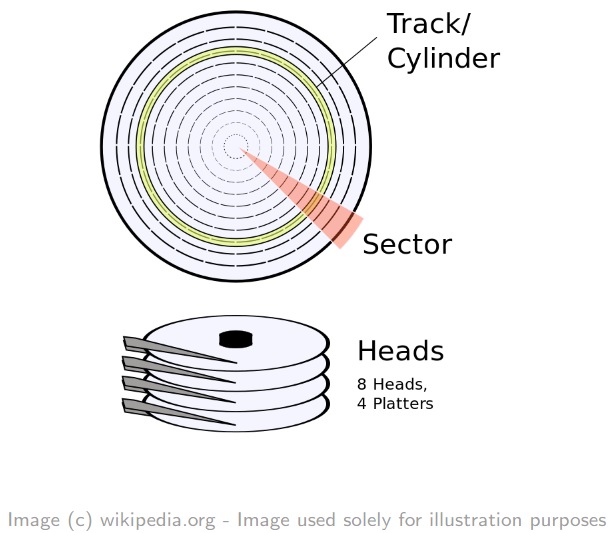
\includegraphics[scale=0.2]{images/chs.png}
        \captionsetup{labelformat=empty,labelsep=none}
        \transparent{0.4}%
        \caption[]{\tiny Image (c) wikipedia.org - Image used solely for illustration purposes}
    \end{figure}
\end{frame}


\begin{frame}[fragile]
  \frametitle{5.3 Low-Level: Sector Structur}
    \begin{figure}
        \includegraphics[scale=0.5]{images/sector.png}
        \captionsetup{labelformat=empty,labelsep=none}
        \transparent{0.4}%
        \caption[]{\tiny Image (c) forensicfocus.com - Image used solely for illustration purposes}
    \end{figure}
\end{frame}


\begin{frame}[fragile]
  \frametitle{5.4 Low-Level: Legacy considerations}
    \begin{itemize}
        \item[] Interleave Factor:
\begin{lstlisting}[basicstyle=\tiny]
Interleave factor 1:1 --> 01 02 03 04 05 06 07 08 09 10 11 12 13 14 15 16 17 
Interleave factor 2:1 --> 01 10 02 11 03 12 04 13 05 14 06 15 07 16 08 17 09 
Interleave factor 3:1 --> 01 07 13 02 08 14 03 09 15 04 10 16 05 11 17 06 12
\end{lstlisting}
        \item[] Zone Bit Recording:
\begin{lstlisting}[basicstyle=\tiny]
   Zone:  12  11  10  09  08  07  06  05  04  03  02  01  00
------------------------------------------------------------
 Tracks: 100 120 140 155 170 185 195 205 210 210 215 218 220
Sectors: 132 132 132 132 132 132 132 132 100 100 100 100 100
------------------------------------------------------------
\end{lstlisting}
        \item[] Head and Cylinder Skewing:
\begin{lstlisting}[basicstyle=\tiny]
No skewing
-----------
Cylinder 0: Head 0: |01 02 03 04 05 06 07 08 09 10 11 12 13 14 15 16 17
	    Head 1: |01 02 03 04 05 06 07 08 09 10 11 12 13 14 15 16 17
Cylinder 1: Head 0: |01 02 03 04 05 06 07 08 09 10 11 12 13 14 15 16 17

Head skew = 1, Cylinder skew = 4
--------------------------------
Cylinder 0: Head 0: |01 02 03 04 05 06 07 08 09 10 11 12 13 14 15 16 17
	    Head 1:  17|01 02 03 04 05 06 07 08 09 10 11 12 13 14 15 16
Cylinder 1: Head 0:  13 14 15 16 17|01 02 03 04 05 06 07 08 09 10 11 12
\end{lstlisting}
    \end{itemize}
\end{frame}


\begin{frame}[fragile]
  \frametitle{5.5 LBA - Logical Block Addressing - Abstract}
  \begin{lstlisting}[basicstyle=\tiny\ttfamily]
Logical volume addresses
----------------------------------------------------------------------------
|  0 |  1 |  2 |  3 |  4 |  5 |  6 |  7 |  8 |  9 | 10 | 11 | 12 | 13 | 14 |
----------------------------------------------------------------------------
          |                   |                   |                   |
          |                   |                   |                   |
          -------------------------------------------------------------
   ^      |         0         |         1         |         3         |   ^
   |      -------------------------------------------------------------   |
   |      Logical file system addresses - Clusters                        |
  MBR                                                               Volume slack
          *-------------------*
               2.048 Bytes
          *-----------------------------------------------------------*
                                   6.144 Bytes
  \end{lstlisting}
\end{frame}


\begin{frame}[fragile]
  \frametitle{5.6 MBR - Master Boot Record}
  \begin{lstlisting}[basicstyle=\tiny]
# dd if=/dev/sdc bs=512 count=1 skip=0 |xxd

0000000: fab8 0010 8ed0 bc00 b0b8 0000 8ed8 8ec0  ................
0000016: fbbe 007c bf00 06b9 0002 f3a4 ea21 0600  ...|.........!..
0000032: 00be be07 3804 750b 83c6 1081 fefe 0775  ....8.u........u
0000048: f3eb 16b4 02b0 01bb 007c b280 8a74 018b  .........|...t..
0000064: 4c02 cd13 ea00 7c00 00eb fe00 0000 0000  L.....|.........
0000080: 0000 0000 0000 0000 0000 0000 0000 0000  ................
0000096: 0000 0000 0000 0000 0000 0000 0000 0000  ................
...
...
0000432: 0000 0000 0000 0000 9af0 0200 0000 0020  ............... 
0000448: 2100 0b1b 0299 0008 0000 0080 2500 00a8  !...........%...
0000464: 01a8 071a b327 0058 2900 00c0 5d00 001a  .....'.X)...]...
0000480: b427 076c dad2 0018 8700 00c0 6800 0000  .'.l........h...
0000496: 0000 0000 0000 0000 0000 0000 0000 55aa  ..............U.



000 - 439       0x000 - 0x1B7    Boot code
440 - 443       0x1B8 - 0x1BB    Disc signature
444 - 445       0x1BC - 0x1BD    Reserved
446 - 509       0x1BE - 0x1FD    Partitiontable
510 - 511       0x1FE - 0x1FF    0x55 0xAA
  \end{lstlisting}
\end{frame}


\begin{frame}[fragile]
  \frametitle{5.6 MBR - DOS Partition Table}
  \begin{lstlisting}[basicstyle=\tiny,escapechar=\*]
# dd if=/dev/sdc bs=512 count=1 skip=0 |xxd

0000000: fab8 0010 8ed0 bc00 b0b8 0000 8ed8 8ec0  ................
0000016: fbbe 007c bf00 06b9 0002 f3a4 ea21 0600  ...|.........!..
0000032: 00be be07 3804 750b 83c6 1081 fefe 0775  ....8.u........u
0000048: f3eb 16b4 02b0 01bb 007c b280 8a74 018b  .........|...t..
0000064: 4c02 cd13 ea00 7c00 00eb fe00 0000 0000  L.....|.........
0000080: 0000 0000 0000 0000 0000 0000 0000 0000  ................
0000096: 0000 0000 0000 0000 0000 0000 0000 0000  ................
...
...
0000432: 0000 0000 0000 0000 9af0 0200 0000 *\underline{0020}*  ............... 
0000448: 2100 0b1b 0299 0008 0000 0080 2500 *\underline{00a8}*  !...........%...
0000464: 01a8 071a b327 0058 2900 00c0 5d00 *\underline{001a}*  .....'.X)...]...
0000480: b427 076c dad2 0018 8700 00c0 6800 *\underline{0000}*  .'.l........h...
0000496: 0000 0000 0000 0000 0000 0000 0000 55aa  ..............U.



Partitiontable:
  Offset: 0     Size: 1	Value: 0x80     --> Bootable
  Offset: 1     Size: 3	Value:          --> Starting CHS address
  Offset: 4     Size: 1	Value: 0x0b     --> FAT32
                               0x07     --> NTFS
  Offset: 5     Size: 3	Value:          --> Ending CHS address
  Offset: 8     Size: 4 Value:          --> Starting LBA address
  Offset:12     Size: 4 Value:          --> LBA size in sectors

  \end{lstlisting}
\end{frame}


\begin{frame}[fragile]
  \frametitle{5.6 MBR - DOS Partition Table}
  \begin{lstlisting}[basicstyle=\tiny,escapechar=\?]
  0000432: 0000 0000 0000 ?\texttt{0000 9af0}? ?\texttt{0200 0000}? 0020  ............... 
  0000448: 2100 0b1b 0299 ?\underline{0008 0000}? ?\underline{0080 2500}? 00a8  !...........%...
  0000464: 01a8 071a b327 ?\underline{0058 2900}? ?\underline{00c0 5d00}? 001a  .....'.X)...]...
  0000480: b427 076c dad2 ?\underline{0018 8700}? ?\underline{00c0 6800}? 0000  .'.l........h...
  0000496: 0000 0000 0000 ?\underline{0000 0000}? ?\underline{0000 0000}? 55aa  ..............U.

Partitiontable:
  Offset: 0     Size: 1	Value: 0x80     --> Bootable
  Offset: 1     Size: 3	Value:          --> Starting CHS address
  Offset: 4     Size: 1	Value: 0x0b     --> FAT32
                               0x07     --> NTFS
  Offset: 5     Size: 3	Value:          --> Ending CHS address
  Offset: 8     Size: 4 Value:          --> Starting LBA address
  Offset:12     Size: 4 Value:          --> LBA size in sectors
  
Addressable space:
  CHS: echo $((2^8 x 2^6 x 2^10 * 512 / 1024^2))  ==  8192 MByte
  LBA: echo $((2^32 * 512 / 1024^3))              ==     2 TByte
  \end{lstlisting}
    \begin{itemize}
	    \item[] Exercise: Calculate the size of the partitions
        \begin{enumerate}
            \item Take 4 byte from "LBA size"
	    \item Switch Little Endian value into Big Endian
	    \item Don't forget: Now you have the sector value, not the byte value
        \end{enumerate}
    \end{itemize}
\end{frame}


\begin{frame}[fragile]
  \frametitle{5.6 MBR - DOS Partition Table}
  \begin{lstlisting}[basicstyle=\tiny,escapechar=\?]
  0000432: 0000 0000 0000 ?\texttt{0000 9af0}? ?\texttt{0200 0000}? 0020  ............... 
  0000448: 2100 0b1b 0299 ?\underline{0008 0000}? ?\underline{0080 2500}? 00a8  !...........%...
  0000464: 01a8 071a b327 ?\underline{0058 2900}? ?\underline{00c0 5d00}? 001a  .....'.X)...]...
  0000480: b427 076c dad2 ?\underline{0018 8700}? ?\underline{00c0 6800}? 0000  .'.l........h...
  0000496: 0000 0000 0000 ?\underline{0000 0000}? ?\underline{0000 0000}? 55aa  ..............U.

  \end{lstlisting}
    \begin{itemize}
	    \item[] Exercise: Calculate the size if the partitions
    \end{itemize}
  \begin{lstlisting}[basicstyle=\tiny]
        Little Endian  Big Endian     Decimal     Sector size
-----------------------------------------------------------------------------
Part1:  0x00802500     0x00258000     2457600     * 512     1258291200   1.2 GB
Part2:  0x00c05d00     0x005dc000     6144000     * 512     3145728000   3.0 GB
Part3:  0x00c06800     0x0068c000     6864896     * 512     3514826752   3.4 GB
  \end{lstlisting}
    \begin{itemize}
        \item Demo:     Change partition type with hexeditor
	\item[] \texttt{fdisk -l /dev/sdb; hexedit /dev/sdb; F2, CTRL+x}
	\item[]
        \item Exercise: Find password in unused space before first partition
    \end{itemize}
\end{frame}


\begin{frame}[fragile]
  \frametitle{5.7 EBR - Extended Partitions}
  \begin{lstlisting}[basicstyle=\tiny]
MBR:  000001b0: 0000 0000 0000 0000 d7b8 0cae 0000 0014
      000001c0: 0904 050f 823e 0008 0000 0000 0400 0000


                           Extended Partition Container                          
------------------------------------------------------------------------------------
|EBR|000|     Logical     |                                                        |
------------------------------------------------------------------------------------
    --->                  ---------------------------
    --------------------> |EBR|000|     Logical     |
    Extended Partition    ---------------------------
                              --->                  ---------------------
    ----------------------------------------------> |EBR|000|  Logical  |
                              Extended Partition    ---------------------
                                                        --->

EBR_01:  001001b0: 0000 0000 0000 0000 0000 0000 0000 0029
         001001c0: 0708 0717 0a2c 0008 0000 0040 0000 0018
         001001d0: 012c 051f 4206 0048 0000 0088 0100 0000

         EBR_02:  00A001B0: 0000 0000 0000 0000 0000 0000 0000 002C
                  00A001C0: 0930 071F 4206 0008 0000 0080 0100 001F
                  00A001D0: 4306 0503 8228 00D0 0100 0008 0200 0000

                  EBR_03:  03B001B0: 0000 0000 0000 0000 0000 0000 0000 0006
                           03B001C0: 410B 0703 8228 0008 0000 0000 0200 0000
                           03B001D0: 0000 0000 0000 0000 0000 0000 0000 0000
  \end{lstlisting}
\end{frame}


\begin{frame}[fragile]
  \frametitle{5.8 GPT - GUID Partition Table}
    \begin{itemize}
        \item BIOS $\to$ UEFI - Unified Extensible Firmware Interface
	\item GUID - Globally Unique Identifier for each partition
	\item[] $\to$ GUID Partition Table
	\item Protective MBR at LBA0
        \begin{itemize}
            \item One single entry covering the entire disk
            \item Partition type 0xEE
	    \item[] if 0xEE unknown $\to$ Not empty $\to$ Not formatted
        \end{itemize}
	\item GPT header at LBA1
	\item GPT entries at LBA2 $\to$ LBA34
	\item GPT entries: 128 Bytes
	\item GPT backup at end of disk
    \end{itemize}
\end{frame}


\begin{frame}[fragile]
  \frametitle{5.8 GPT - GUID Partition Table}
    \begin{figure}
        \caption[]{\tiny Image (c) wikipedia.org - Image used solely for illustration purposes}
	    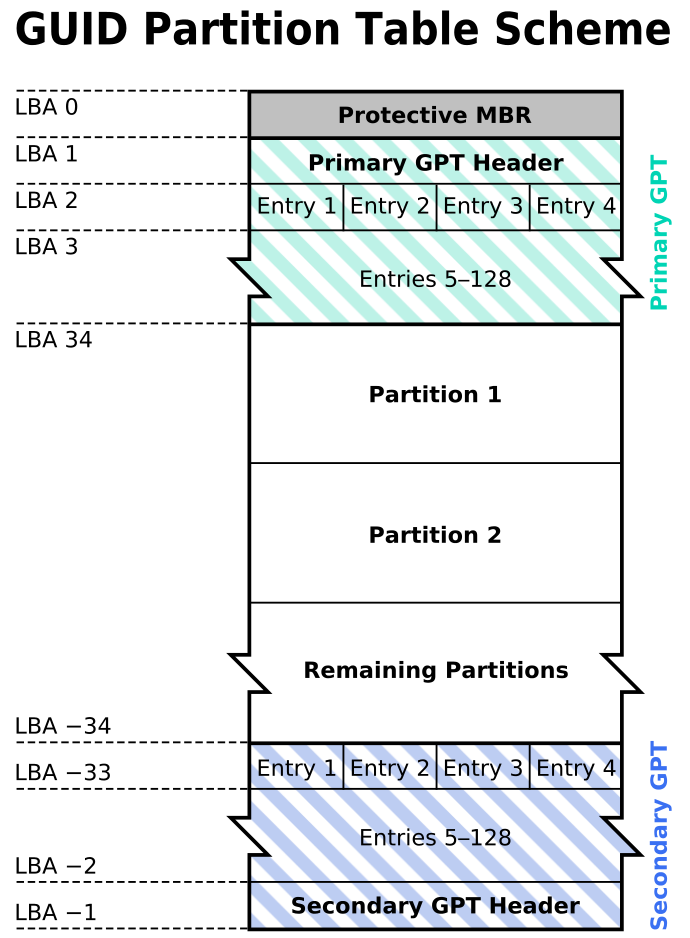
\includegraphics[scale=0.23,angle=270]{images/gpt.png}
        \captionsetup{labelformat=empty,labelsep=none}
        \transparent{0.4}%
    \end{figure}
\end{frame}


\begin{frame}[fragile]
  \frametitle{5.9 VBR - Volume Boot Record - Boot Sector}
  \begin{lstlisting}[basicstyle=\tiny]
# dd if=/dev/sdc1 bs=512 count=1 skip=0 |xxd

0000000: eb58 906d 6b64 6f73 6673 0000 0208 2000  .X.mkdosfs.... .     # 0xeb 0x58 0x90
0000010: 0200 0000 00f8 0000 3e00 f800 0000 0000  ........>.......     # JMP  2+88 NOP
0000030: 0100 0600 0000 0000 0000 0000 0000 0000  ................
0000040: 0000 29a2 20e9 9c46 4154 2020 2020 2020  ..). ..FAT      
0000050: 2020 4641 5433 3220 2020 0e1f be77 7cac    FAT32   ...w|.
0000060: 22c0 740b 56b4 0ebb 0700 cd10 5eeb f032  ".t.V.......^..2
...
...
00001f0: 0000 0000 0000 0000 0000 0000 0000 55aa  ..............U.


0 - 2           Size:  3    Jump to bootstrap code
3 - 10          Size:  8    OEM-ID: mkdosfs
11 - 12         Size:  2    Bytes per sector: 0x0002 -> 0x0200 (little endian)-> 512
13 (0xD)        Size:  1    Sectors per cluster: 0x08 -> 4096 bytes per cluster
50 (0x32) - 51  Size:  2    Boot sector backup: 0x0600 -> 0x0006 -> at sector 6
67 (0x43) - 70  Size:  4    Volume serial number: 0xa220e99c -> 0x9ce920a2
71 (0x47)       Size: 11    Volume label: FAT
82 (0x52)       Size:  8    Partition type: FAT32
90 (0x5A)- 509 (0x1FD)	    Bootstrap code
510 (0x1FE)     Size:  2    Signature: 0x55AA
  \end{lstlisting}
    \begin{itemize}
        \item Demo: Sleuthkit tools: \texttt{mmstat, mmls, fsstat}
    \end{itemize}
\end{frame}





%
% This work is licensed under a Creative Commons Attribution-ShareAlike 4.0 International License.
% http://creativecommons.org/licenses/by-sa/4.0/
%

% DO NOT COMPILE THIS FILE DIRECTLY!
% This is included by the other .tex files.


\begin{frame}
    \includegraphics[scale=0.3]{images/logo-circl-Forensics.png}
    \begin{itemize}
        \item[]
        \item[]
        \item[] 6. Forensics Challenges
    \end{itemize}
\end{frame}


\begin{frame}[fragile]
  \frametitle{6.1 Hide and recover data}
  \begin{itemize}
    \item Situation:
    \begin{itemize}
      \item USB stick image
      \item One partition
      \item Several unallocated sectors
      \item[]
    \end{itemize}
    \item Challenge:
    \begin{itemize}
      \item Hide a message in unallocated sector
      \item Recover the message
      \item Hide a binary in unallocated sectors
      \item Recover the binary
      \item[]
    \end{itemize}
    \item Hiding Data outside the file system
    \begin{itemize}
	    \item[] \url{https://cyberday.lu/wp-content/uploads/2024/10/05\_CIRCL\_CyberDayLu2024.pdf} 
      \item[]
    \end{itemize}
  \end{itemize}
\end{frame}


\begin{frame}[fragile]
  \frametitle{6.2 Recovering corrupt MBR}
  \begin{itemize}
    \item Situation:
    \begin{itemize}
      \item USB stick image
      \item Several partitions available
      \item At least one partition do not mount
      \item[]
    \end{itemize}
    \item Challenge:
    \begin{itemize}
      \item Examine the partition table
      \item Find the first sector of the partition
      \item Fix the Master Boot Record - MBR
      \item Analyze the other offsets
      \item Analyze unallocated sectors
      \item[]
    \end{itemize}
  \end{itemize}
\end{frame}


\begin{frame}[fragile]
  \frametitle{6.2 Recovering corrupt MBR}
  \begin{lstlisting}[basicstyle=\tiny]
1. Examine the partition table
------------------------------
    $ fdisk -l mbr/mbr_ex.raw 
        Sector size (logical/physical): 512 bytes / 512 bytes
        Disklabel type: dos
        Disk identifier: 0x9392806f

        Device          Boot  Start    End Sectors Size Id Type
        mbr/mbr_ex.raw1        2050  67585   65536  32M  c W95 FAT32 (LBA)
        mbr/mbr_ex.raw2       67586 133119   65534  32M  c W95 FAT32 (LBA)
        mbr/mbr_ex.raw3      133120 262142  129023  63M  c W95 FAT32 (LBA)
  
  
    $ mmls mbr/mbr_ex.raw
        DOS Partition Table
        Offset Sector: 0
        Units are in 512-byte sectors

              Slot      Start        End          Length       Description
        000:  Meta      0000000000   0000000000   0000000001   Primary Table (#0)
        001:  -------   0000000000   0000002049   0000002050   Unallocated
        002:  000:000   0000002050   0000067585   0000065536   Win95 FAT32 (0x0c)
        003:  000:001   0000067586   0000133119   0000065534   Win95 FAT32 (0x0c)
        004:  000:002   0000133120   0000262142   0000129023   Win95 FAT32 (0x0c)
        005:  -------   0000262143   0000262143   0000000001   Unallocated
  \end{lstlisting}
\end{frame}


\begin{frame}[fragile]
  \frametitle{6.2 Recovering corrupt MBR}
  \begin{lstlisting}[basicstyle=\tiny]
2. Investigate start of 1th partition
-------------------------------------
    dd if=mbr/mbr_ex.raw skip=2050 count=1 status=none | xxd | less
    dd if=mbr/mbr_ex.raw skip=2047 count=4 status=none | xxd | less


Fix LBA Start vaule of 1th partition entry
------------------------------------------
    Calculation: 2048 = 0x00000800 => little endian: 0X00080000
        Replace 0X02080000 with 0X00080000

    hexedit -l 16 mbr/mbr_ex.raw
        000001C0   21000C34  30040008  00000000  01000033


Review partition table and file system stats
--------------------------------------------
    mmls mbr/mbr_ex.raw 
              Slot      Start        End          Length       Description
        000:  Meta      0000000000   0000000000   0000000001   Primary Table (#0)
        001:  -------   0000000000   0000002047   0000002048   Unallocated
        002:  000:000   0000002048   0000067583   0000065536   Win95 FAT32 (0x0c)
        003:  -------   0000067584   0000067585   0000000002   Unallocated
        004:  000:001   0000067586   0000133119   0000065534   Win95 FAT32 (0x0c)
        005:  000:002   0000133120   0000262142   0000129023   Win95 FAT32 (0x0c)
        006:  -------   0000262143   0000262143   0000000001   Unallocated
  \end{lstlisting}
\end{frame}


\begin{frame}[fragile]
  \frametitle{6.2 Recovering corrupt MBR}
  \begin{lstlisting}[basicstyle=\tiny]
3. Investigate end of 1th and start of 2nd partition
----------------------------------------------------
    fsstat -o 2048 mbr/mbr_ex.raw
        File System Type: FAT16
        Total Range: 0 - 65535
	....
	--> Size of partition 1 is okay


    sigfind -o 510 -l AA55 mbr/mbr_ex.raw
        Block: 0 (-)
        Block: 2048 (+2048)
        Block: 67586 (+65538)
        Block: 133120 (+65534)


    fsstat -o 67586 mbr/mbr_ex.raw
        File System Type: FAT16
        Total Range: 0 - 65533
        ....
	--> Start of partition 2 is okay
	--> There are 2 unallocated sectors in between
	--> Size of partition 2 is okay 


Investigate the sectors
-----------------------
    dd if=mbr/mbr_ex.raw skip=67583 count=4 | xxd | less
  \end{lstlisting}
\end{frame}


\begin{frame}[fragile]
  \frametitle{6.2 Recovering corrupt MBR}
  \begin{lstlisting}[basicstyle=\tiny]
        005:  000:002   0000133120   0000262142   0000129023   Win95 FAT32 (0x0c)
        006:  -------   0000262143   0000262143   0000000001   Unallocated

  
4. Investigate 3rd partition
----------------------------
    sigfind -o 510 -l AA55 mbr/mbr_ex.raw
        Block: 0 (-)
        Block: 2048 (+2048)
        Block: 67586 (+65538)
        Block: 133120 (+65534)


    fsstat -o 133120 mbr/mbr_ex.raw
        File System Type: FAT16
        Total Range: 0 - 129022
        ....
	--> Start of partition 3 is okay
	--> Size of partition 3 is okay 
	--> There is 1 unallocated sector at end of disk


Investigate the last 2 sectors of disk
--------------------------------------
    dd if=mbr/mbr_ex.raw skip=262142 | xxd | less
  \end{lstlisting}
\end{frame}


\begin{frame}[fragile]
    \frametitle{6.3 Lost in Hyperspace: USB stick investigation}
  \begin{itemize}
    \item Situation:
    \begin{itemize}
      \item USB stick image with one extended partition
      \item Some logical partitions available
      \item Countles partitions get mounted
      \item[]
    \end{itemize}
    \item Challenge:
    \begin{itemize}
      \item Analyze USB stick with standard tools
      \item Analyze MBR with a hexeditor
      \item Discover whats going wrong
      \item Fix the broken values
      \item[]
    \end{itemize}
  \end{itemize}
\end{frame}


\begin{frame}[fragile]
    \frametitle{6.3 Lost in Hyperspace: USB stick investigation}
    \begin{itemize}
            \item[] USB stick before manipulation:
\begin{lstlisting}[basicstyle=\tiny\ttfamily]
# dmesg -T
     [Do Jan 23 21:40:07 2020] sd 1:0:0:0: [sdb] 250068992 512-byte logical blocks: 
     [Do Jan 23 21:40:07 2020]  sdb: sdb1 < sdb5 sdb6 sdb7 >

# fdisk -l /dev/sdb
     Device     Boot  Start    End Sectors  Size Id Type
     /dev/sdb1         2048 264191  262144  128M  5 Extended
     /dev/sdb5         4096  20479   16384    8M  7 HPFS/NTFS/exFAT
     /dev/sdb6        22528 120831   98304   48M  7 HPFS/NTFS/exFAT
     /dev/sdb7       122880 253951  131072   64M  7 HPFS/NTFS/exFAT

# mount              /dev/sdb7 on /media/michael/DFIR
                     /dev/sdb6 on /media/michael/CIRCL
                     /dev/sdb5 on /media/michael/test

# df -ha | grep sdb
     /dev/sdb7             64M  2,5M   62M   4% /media/michael/DFIR
     /dev/sdb6             48M  2,5M   46M   6% /media/michael/CIRCL
     /dev/sdb5            8,0M  2,5M  5,6M  31% /media/michael/test
\end{lstlisting}
            \item[] Manipulation 4 bytes:
\begin{lstlisting}[basicstyle=\tiny\ttfamily]
# hexedit /dev/sdb
     .....
     03B001C0   41 0B 07 03  82 28 00 08  00 00 00 00  02 00 00 00  A....(..........
     03B001D0   00 00 05 00  00 00 00 48  00 00 00 88  01 00 00 00  .......H........
\end{lstlisting}
    \end{itemize}
\end{frame}


\begin{frame}[fragile]
    \frametitle{6.3 Lost in Hyperspace: WTF}
    \includegraphics[scale=0.2]{images/ebr.png}
\end{frame}


\begin{frame}[fragile]
    \frametitle{6.3 Lost in Hyperspace: USB stick investigation}
  \begin{lstlisting}[basicstyle=\tiny]
$ fdisk -l /dev/sdb

     Device        Boot  Start    End Sectors  Size Id Type
     /dev/sdb1            2048 264191  262144  128M  5 Extended
     /dev/sdb5            4096  20479   16384    8M  7 HPFS/NTFS/exFAT
     /dev/sdb6           22528 120831   98304   48M  7 HPFS/NTFS/exFAT
     /dev/sdb7          122880 253951  131072   64M  7 HPFS/NTFS/exFAT
     /dev/sdb8           22528 120831   98304   48M  7 HPFS/NTFS/exFAT
     /dev/sdb9          122880 253951  131072   64M  7 HPFS/NTFS/exFAT
          .....
          .....
     /dev/sdb56          22528 120831   98304   48M  7 HPFS/NTFS/exFAT
     /dev/sdb57         122880 253951  131072   64M  7 HPFS/NTFS/exFAT
     /dev/sdb58          22528 120831   98304   48M  7 HPFS/NTFS/exFAT
     /dev/sdb59         122880 253951  131072   64M  7 HPFS/NTFS/exFAT
     /dev/sdb60          22528 120831   98304   48M  7 HPFS/NTFS/exFAT

$ mount
          .....
     /dev/sdb79 on /media/michael/DFIR25
     /dev/sdb82 on /media/michael/CIRCL28
     /dev/sdb86 on /media/michael/CIRCL33 
          .....
          .....
     /dev/sdb162 on /media/michael/CIRCL68
     /dev/sdb163 on /media/michael/DFIR73
     /dev/sdb166 on /media/michael/CIRCL64
  \end{lstlisting}
\end{frame}


\begin{frame}[fragile]
    \frametitle{6.3 Lost in Hyperspace: USB stick investigation}
    \begin{itemize}
	    \item[] Do further investigations:
  \begin{lstlisting}[basicstyle=\tiny]
$ df -ha

          .....
     /dev/sdb157           64M  2,5M   62M   4% /media/michael/DFIR72
     /dev/sdb158           48M  2,5M   46M   6% /media/michael/CIRCL63
     /dev/sdb159           64M  2,5M   62M   4% /media/michael/DFIR69
     /dev/sdb160           48M  2,5M   46M   6% /media/michael/CIRCL67
     /dev/sdb162           48M  2,5M   46M   6% /media/michael/CIRCL68
     /dev/sdb163           64M  2,5M   62M   4% /media/michael/DFIR73
          .....


$ mmls /dev/sdb                         --> Nothing... WTF?


  \end{lstlisting}
	    \item[] Any ideas how to proceed?
	    \item[] $\to$ Use hexeditor to read the partition table
    \end{itemize}
\end{frame}


\begin{frame}[fragile]
    \frametitle{6.3 Lost in Hyperspace: Solution step 1}
  \begin{lstlisting}[basicstyle=\tiny]
                           Extended Partition Container                          
------------------------------------------------------------------------------------
|EBR|000|     Logical     |                                                        |
------------------------------------------------------------------------------------
    --->                  ---------------------------
    --------------------> |EBR|000|     Logical     |
    Extended Partition    ---------------------------
                              --->                  ---------------------
                              --------------------> |EBR|000|  Logical  |
                              Extended Partition    ---------------------
                                                        --->



EBR_01:  001001b0: 0000 0000 0000 0000 0000 0000 0000 0029
         001001c0: 0708 0717 0a2c 0008 0000 0040 0000 0018
         001001d0: 012c 051f 4206 0048 0000 0088 0100 0000

         EBR_02:  00A001B0: 0000 0000 0000 0000 0000 0000 0000 002C
                  00A001C0: 0930 071F 4206 0008 0000 0080 0100 001F
                  00A001D0: 4306 0503 8228 00D0 0100 0008 0200 0000

                  EBR_03:  03B001B0: 0000 0000 0000 0000 0000 0000 0000 0006
                           03B001C0: 410B 0703 8228 0008 0000 0000 0200 0000
                           03B001D0: 0000 0000 0000 0000 0000 0000 0000 0000
  \end{lstlisting}
\end{frame}


\begin{frame}[fragile]
    \frametitle{6.3 Lost in Hyperspace: Solution step 2}
\begin{lstlisting}[basicstyle=\tiny]
                           Extended Partition Container                          
------------------------------------------------------------------------------------
|EBR|000|     Logical     |                                                        |
------------------------------------------------------------------------------------
    --->                  ---------------------------
    --------------------> |EBR|000|     Logical     |
    Extended Partition    ---------------------------
                              --->                  ---------------------
                              --------------------> |EBR|000|  Logical  |
                              Extended Partition    ---------------------
                                                        --->
                           <-----------------------------


EBR_01:  001001b0: 0000 0000 0000 0000 0000 0000 0000 0029
         001001c0: 0708 0717 0a2c 0008 0000 0040 0000 0018
         001001d0: 012c 051f 4206 0048 0000 0088 0100 0000

         EBR_02:  00A001B0: 0000 0000 0000 0000 0000 0000 0000 002C
                  00A001C0: 0930 071F 4206 0008 0000 0080 0100 001F
                  00A001D0: 4306 0503 8228 00D0 0100 0008 0200 0000

                  EBR_03:  03B001B0: 0000 0000 0000 0000 0000 0000 0000 0006
                           03B001C0: 410B 0703 8228 0008 0000 0000 0200 0000
                           03B001D0: 0000 0500 0000 0048 0000 0088 0100 0000
  \end{lstlisting}
\end{frame}





\include{f19_bib}

\begin{frame}
  \frametitle{Overview}
  \begin{itemize}
  \item[]
      \begin{enumerate}
          \item Introduction
          \item Information
          \item Disk Acquisition
          \item Disk Cloning / Disk Imaging
          \item Disk Analysis
          \item Forensics Challenges
          \item Bibliography and Outlook
      \end{enumerate}
  \end{itemize}
\end{frame}

\end{document}

